\RequirePackage[l2tabu, orthodox]{nag}
%\documentclass[12pt]{article}
\documentclass[preprint,12pt,times]{elsarticle}

\biboptions{sort&compress,comma,square}

% \usepackage{url}

% \usepackage[linesnumbered,lined,commentsnumbered,ruled]{algorithm2e}
%\usepackage{amssymb}
\usepackage{amsmath}
%\usepackage{amsfonts}
\usepackage{bm}
%\usepackage{bbm}
%\usepackage{caption}
\usepackage{xcolor}
%\usepackage{geometry}
%\usepackage{graphicx}
%\usepackage[colorlinks,linkcolor=blue,citecolor=blue,urlcolor=blue]{hyperref}
\usepackage{listings}
\lstset{ %
   backgroundcolor=\color{white},   % choose the background color; you must add \usepackage{color} or \usepackage{xcolor}
   basicstyle=\small,        % the size of the fonts that are used for the code
   breakatwhitespace=false,         % sets if automatic breaks should only happen at whitespace
   breaklines=false,                 % sets automatic line breaking
   captionpos=b,                    % sets the caption-position to bottom
   %commentstyle=\color{mygreen},    % comment style
   deletekeywords={...},            % if you want to delete keywords from the given language
   escapeinside={\%*}{*)},          % if you want to add LaTeX within your code
   extendedchars=false,              % lets you use non-ASCII characters; for 8-bits encodings only, does not work with UTF-8
   frame=single,	                   % adds a frame around the code
   keepspaces=true,                 % keeps spaces in text, useful for keeping indentation of code (possibly needs columns=flexible)
   keywordstyle=\color{blue},       % keyword style
   language=C++,                 % the language of the code
   otherkeywords={*,...},           % if you want to add more keywords to the set
   numbers=left,                    % where to put the line-numbers; possible values are (none, left, right)
   numbersep=5pt,                   % how far the line-numbers are from the code
   numberstyle=\tiny\color{gray}, % the style that is used for the line-numbers
   rulecolor=\color{black},         % if not set, the frame-color may be changed on line-breaks within not-black text (e.g. comments (green here))
   showspaces=false,                % show spaces everywhere adding particular underscores; it overrides 'showstringspaces'
   showstringspaces=false,          % underline spaces within strings only
   showtabs=false,                  % show tabs within strings adding particular underscores
   stepnumber=2,                    % the step between two line-numbers. If it is 1, each line will be numbered
%   stringstyle=\color{mymauve},     % string literal style
   tabsize=2,	                   % sets default tabsize to 2 spaces
   title=\lstname                   % show the filename of files included with \lstinputlisting; also try caption instead of title
}
%\usepackage{layouts}
%\usepackage{mathrsfs}
%\usepackage{pgfkeys,pgfmath,pgfcore}
%\usepackage{srcltx}
%\usepackage[labelformat=simple]{subcaption}
%\usepackage{xspace}
\usepackage[linesnumbered,lined,commentsnumbered,ruled]{algorithm2e}

\usepackage[format=plain,indention=.5cm]{caption}
\usepackage[labelformat=simple]{subcaption}
\renewcommand\thesubfigure{(\alph{subfigure})}

%\renewcommand{\thetable}{\arabic{table}}
%\captionsetup[table]{labelformat=simple, labelsep=colon}

%\pgfkeys{/pgf/number format/.cd,1000 sep={}}

%% see http://tex.stackexchange.com/questions/2441/how-to-add-a-forced-line-break-inside-a-table-cell
%\newcommand{\specialcell}[2][c]{%
%  \begin{tabular}[#1]{@{}c@{}}#2\end{tabular}}

% put your own definitions here:
% \renewcommand\thesubfigure{(\alph{subfigure})}
\def\gz  #1{           \mbox{$\boldsymbol{#1}$}}
% \DeclareMathAlphabet{\bsf}{OT1}{cmss}{bx}{n}
% \def\msf  #1{           \mbox{\!\!      $\sf #1$}}
\def\Grad #1 {{\rm Grad} #1}
\def\grad {\mbox{grad}}
\def\Div {\mbox{Div\,}}
\def\div {\mbox{div\,}}
\def\d {\mbox{d}}
\def\D {\mbox{D}}
% \newcommand{\norm}[1]{\left\lvert #1 \right\rvert}
%\newcommand\normDouble[1]{\left\lVert#1\right\rVert}
%\newcommand{\normXY}[1]{\lvert #1 \rvert_{2d}}
%\newcommand{\dbracket}[1]{\left[\!\!\left[ #1 \right]\!\!\right]}

\def\mcl  #1{               {\cal #1}}
%\def\bcl  #1{\mbox{\boldmath$\cal #1$}}

%\DeclareMathOperator{\det}{det}
\DeclareMathOperator{\trace}{tr}
\newcommand{\diff}{\mathop{}\!\mathrm{d}}


\begin{document}

\begin{frontmatter}
  \title{
  A matrix-free approach for finite-strain hyperelastic problems using geometric multigrid
  }

  \author[a]{Denis Davydov\corref{cor}}
  \ead{denis.davydov@fau.de}

  \author[a]{Jean-Paul Pelteret}
  \ead{jean-paul.pelteret@fau.de}

  \author[b]{Daniel Arndt}
  \ead{daniel.arndt@iwr.uni-heidelberg.de}

  \author[a,c]{Paul Steinmann}
  \ead{paul.steinmann@fau.de}

  \cortext[cor]{Corresponding author.}

  \address[a]{Chair of Applied Mechanics,
  Friedrich-Alexander-Universit\"{a}t Erlangen-N\"{u}rnberg,
  Egerlandstr.\ 5, 91058 Erlangen, Germany}

  \address[b]{Interdisciplinary Center for Scientific Computing (IWR),
      Heidelberg University,
      Im Neuenheimer Feld 205,
      69120 Heidelberg,
      Germany}

  \address[c]{Glasgow computational engineering center,
      University of Glasgow, G12 8QQ Glasgow, United Kingdom
  }


  \begin{abstract}
    The performance of finite element solvers on modern computer architectures is typically memory bound.
    The main cause for this is that loading matrix elements from RAM into CPU cache is significantly slower than performing the arithmetic operations when solving the problem.
    In order to improve the performance of iterative solvers within the high-performance computing context, so-called matrix-free methods are
    widely adopted in the fluid mechanics community, where matrix-vector products are computed on-the-fly.

    In this work, we extend the application of matrix-free approaches to problems in solid mechanics and investigate different implementations of the finite-strain hyperelastic tangent operator numerically.
    In order to improve the convergence behavior of iterative solvers, we also propose a method by which to construct level tangent operators
    and employ them to define a geometric multigrid preconditioner.
    Our implementation employs MPI and Intel Threading Building Blocks parallelization, and SIMD vectorization.
    The performance of the matrix-free operator and the geometric multigrid preconditioner is compared to the matrix-based implementation with an algebraic multigrid preconditioner for a representative numerical example of a heterogeneous hyperelastic material in two and three dimensions.
  \end{abstract}


  \begin{keyword}
      adaptive finite element method \sep
      geometric multigrid \sep
      finite-strain \sep
      matrix-free \sep
      hyperelasticity
  \end{keyword}

  \end{frontmatter}

\section{Introduction}

The performance of finite element solvers on modern computer architectures is typically memory bound.
The main cause for this is that loading pre-computed matrix elements from RAM into CPU cache is significantly slower than performing the arithmetic operations when solving the problem.
In order to improve the performance of iterative solvers, so-called matrix-free methods,
where matrix-vector products are formed on-the-fly \cite{kronbichler12,May2015, Krank2017, Brown2010, Gmeiner2016},
are widely adopted in the fluid mechanics community.
Such methods can also be efficiently implemented on GPUs \cite{Abdelfattah2016, ljungkvist2017multigrid}.

To the best of our knowledge, matrix-free methods are not widely adopted within the solid mechanics community.
We are only aware of a single paper currently in preparation that deals with small strain linear elasticity \cite{Clevenger2018} and a recent masters thesis produced by a student of the first two of the authors \cite{Mentler2017}.
One possible reason is that the tangent operators (stemming from linearization of the nonlinear balance equations) are
more elaborate as compared to the operators used often in both linear and non-linear fluid mechanics, and it is not obvious whether the matrix-free methods can be advantageous in this case.
Another reason could be the use of lower order elements due to lacking smoothness of the underlying solution.
The finite element method (FEM) with linear or quadratic elements (that reduce the potential for locking), or mixed or enhanced formulations (that avoid locking) are often adopted in the solid mechanics community.
Even higher order elements are rarely employed.
However, we note that, even with linear FEM, large scale computations with $10^{12}$ unknowns inevitably require a matrix-free approach as there is simply not enough memory to store the sparse tangent matrix \cite{Gmeiner2016}. Therefore, we believe that for large scale computations in solid mechanics it is crucial to consider matrix-free approaches and develop efficient multigrid solvers.

In this work, we investigate different implementations of the finite-strain hyperelastic tangent operator with respect to their computational cost.
In order to improve the convergence of iterative solvers, we also propose a method by which to construct level matrix-free tangent operators
and employ them to define a \mbox{geometric} multigrid preconditioner.
Our implementation employs MPI and Intel Threading Building Blocks parallelization, together with SIMD vectorization.

The paper is organized as follows: In Section \ref{sec:theory} we briefly introduce the partial differential equations used in  finite-strain solid mechanics. Sections \ref{sec:fe} and \ref{sec:mf} cover the finite element discretization and the different matrix-free operator evaluation approaches. In Section \ref{sec:gmg} we propose a geometric multigrid preconditioner suitable for finite-strain hyperelasticity. The performance of the matrix-free operator and the geometric multigrid preconditioner is compared to the matrix-based implementation with an algebraic multigrid preconditioner for a representative numerical example of a heterogeneous hyperelastic material simulated in two and three dimensions in Section \ref{sec:example}. The results are summarized in Section \ref{sec:summary}.

\section{Theoretical background}
\label{sec:theory}

\subsection{Weak form}
%
% Kinematics
%
The deformation of a body $\mcl B$ from the reference configuration $\mcl B_0$ to the current configuration $\mcl B_t$ at time $t$
is defined via the deformation map $\gz \varphi_t: \mcl B_0 \rightarrow \mcl B_t$, which places material points of $\mcl B$ into the Euclidean space $\mathbb E^3$.
The current location of a material particle $\gz X$ is given by $\gz x = \gz \varphi_t (\gz X)$.
The displacement field reads $\gz u = \gz x - \gz X$.

%
% Deformation gradient
%
The tangent map is linear such that
$\d \gz x = \gz F \cdot \d \gz X$,
where $\gz F := \Grad \, \gz \varphi \equiv \gz I + \Grad \, \gz u$ is called deformation gradient and $\gz I$ is the second-order unit tensor.
The mapping has to be one-to-one and must exclude self-penetration. Consequently, the Jacobian $J = \det \gz F > 0$ has to be positive.
% The deformation gradient can be split into the proper orthogonal rotation tensor $\gz R$ and the symmetric right $\gz U$ and left $\gz V$ stretch tensors such that $\gz F = \gz R \gz U = \gz V \gz R$.
We shall denote the push-forward transformation of rank-2 and rank-4 tensors $\mathbf{A}$ and $\boldsymbol{\mathcal{A}}$ by
\begin{align}
  \varphi\left( \mathbf{A} \right)_{ij}
  &= F_{iA} A_{AB} F_{jB} \\
\varphi\left( \boldsymbol{\mathcal{A}} \right)_{ijkl}
  &= F_{iA} F_{jB} \mathcal{A}_{ABCD} F_{kC} F_{lD}.
\end{align}

%
% strain measures
%
In what follows, we parameterize the material behavior using the right Cauchy-Green tensor $\gz C := \gz F^T \cdot \gz F$.
We will also use the Green-Lagrange strain tensor $\gz E:=\frac{1}{2}\left[\gz C - \gz I\right]$ and the left Cauchy-Green tensor $\gz b := \gz F \cdot \gz F^T$.
Clearly $J = \sqrt{\det \gz C}$ and $\partial (\bullet)/\partial \gz E = 2\, \partial (\bullet)/\partial \gz C$.
%
For conservative systems without body forces, the total potential energy functional $\mcl E$ is introduced as
\begin{align}
\mcl E =
\int_{\mcl B_0} \mcl \psi(\gz F) \, \d V \,
- \int_{\partial \mcl B_0^N} \overline{\gz T} \cdot \gz u \, \d S \, ,
\end{align}
where $\overline{\gz T}$ is the prescribed loading at the Neumann part of the boundary $\partial \mcl B_0^N$ in the reference configuration, $\mcl \psi$ denotes the strain-energy per unit reference volume and $\gz u$ should satisfy the prescribed Dirichlet boundary conditions $\gz u = \overline{\gz u}$ on $\partial \mcl B_0^D := \partial \mcl B_0 \setminus \partial \mcl B_0^N \neq \emptyset $.

The principle of stationary potential energy at equilibrium requires that the directional derivative with respect to the displacement
\begin{align}
\delta \mcl E =
\frac{\d}{\d \epsilon} \mcl E (\gz u + \epsilon \delta \gz u) \Bigr\rvert_{\epsilon=0}  = 0 \, .
\label{eq:stationary}
\end{align}
vanishes for all directions $\delta \gz u$ which satisfy homogeneous Dirichlet boundary conditions.
%
This leads to the following scalar non-linear equation
\begin{align}
F(\gz u, \delta \gz u) =
\int_{\mcl B_0} \gz P : \Grad \, \delta \gz u \, \d V \,
-
\int_{\partial \mcl B_0^N} \overline{\gz T} \cdot \delta \gz u \, \d S
= 0 \, ,
\end{align}
where $\gz P := \partial \mcl \psi / \partial \gz F$ is the Piola stress tensor.
The double contraction in the first term can be re-written in terms of the symmetric Kirchhoff stress tensor $\gz \tau := \gz P \cdot \gz F^T$ as
\begin{align}
\gz P : \Grad \, \delta \gz u =
\left[\gz \tau \cdot \gz F^{-T}\right] : \Grad \, \delta \gz u =
\gz \tau : \left[\Grad \, \delta \gz u \cdot \gz F^{-1}\right] =
\gz \tau : \grad \, \delta \gz u \, ,
\end{align}
and therefore
\begin{align}
  F(\gz u, \delta \gz u) =
  \int_{\mcl B_0} \gz \tau : \grad^{s} \, \delta \gz u \, \d V \,
  -
  \int_{\partial \mcl B_0^N} \overline{\gz T} \cdot \delta \gz u \, \d S
  = 0 \, ,
\label{eq:weak_form}
\end{align}
where $\grad^{s} \, \delta \gz u := \frac{1}{2}\left[ \grad \, \delta \gz u + ( \grad \, \delta \gz u)^T\right]$.
Note that $\gz \tau$ is the push-forward transformation of the Piola-Kirchhoff stress $\gz S := \partial \mcl \psi / \partial \gz E \equiv 2 \partial \mcl \psi / \partial \gz C$,
that is $\gz \tau = \varphi(\gz S) = \gz F \cdot \gz S \cdot \gz F^T$.

\subsection{Linearization}

In order to solve \eqref{eq:weak_form} using Newton's method, a first order approximation around a given solution field $\overline{\gz u}$ is required such that
\begin{align}
F(\overline{\gz u} + \Delta \gz u, \delta \gz u) \approx
F(\overline{\gz u}, \delta \gz u) + \D_{\Delta \gz u} F(\overline{\gz u}, \delta \gz u).
\end{align}
For conservative traction boundary conditions, the directional derivative is given by
\begin{align}
\D_{\Delta \gz u}  F(\overline{\gz u}, \delta \gz u)
=
\int_{\mcl B_0} \D_{\Delta \gz u} \gz \tau : \overline{\grad^s} \, \delta \gz u \, \d V
+
\int_{\mcl B_0} \overline{\gz \tau} : \left[ \Grad \, \delta \gz u \cdot \D_{\Delta \gz u}  \gz F^{-1} \right] \d V.
\end{align}
Following \cite{Wriggers2008}, this can be simplified to
\begin{align}
\D_{\Delta \gz u} F(\overline{\gz u}, \delta \gz u)
  =
  \int_{\mcl B_0} \overline{\grad^s} \Delta \gz u : J \boldsymbol{\mathcal{C}} : \overline{\grad^s} \, \delta \gz u \, \d V
  +
  \int_{\mcl B_0}
  \overline{\grad}\delta \gz u :
  \left[
  \overline{\grad} \Delta \gz u \cdot
  \overline{\gz \tau}
  \right]
  \d V.
\label{eq:tangent}
\end{align}
Here $\overline{(\bullet)}$ is used to denote quantities evaluated using the displacement field $\overline {\gz u}$, and the fourth-order tangent tensor is the push forward of the material tangent $J \boldsymbol{\mathcal{C}} = \varphi\left( 4 \frac{d^{2} \psi \left( \mathbf{C} \right)}{d \mathbf{C} \otimes d \mathbf{C}} \right)$. The first term in \eqref{eq:tangent} is related to the linearization of the Kirchhoff stress and therefore called material part of the tangent operator.  The second term in \eqref{eq:tangent} is called geometric part of the tangent since it originates from the linearization of the inverse of the deformation gradient $\gz F^{-1}$.

\subsection{Constitutive modelling}

For the current study, we use the Neo-Hookean model
\begin{gather}
\psi \left( \mathbf{C} \right)
  = \frac{\mu}{2} \left[ \trace{\mathbf{C}} - \trace{\mathbf{I}} - 2 \ln\left( J \right) \right]
  + \lambda \ln^{2}\left( J \right)
\end{gather}
where $\mu$ and $\lambda$ denote the shear modulus and Lam\'{e} parameter respectively. It can be shown that the first and second derivatives of the strain energy function are given by
\begin{align}
\frac{d \psi \left( \mathbf{C} \right)}{d \mathbf{C}}
  &= \frac{\mu}{2} \mathbf{I} - \frac{1}{2} \left[ \mu - 2\lambda\ln\left( J \right) \right] \mathbf{C}^{-1} \\
\frac{d^{2} \psi \left( \mathbf{C} \right)}{d \mathbf{C} \otimes d \mathbf{C}}
  &= \frac{1}{2}\left[ \mu - 2\lambda\ln\left( J \right) \right] \left[ - \frac{d \mathbf{C}^{-1}}{d \mathbf{C}} \right]
  + \frac{\lambda}{2} \mathbf{C}^{-1} \otimes \mathbf{C}^{-1}
\end{align}
The Kirchhoff stress and its associated material tangent are
\begin{gather}
\boldsymbol{\tau}
  \equiv J \boldsymbol{\sigma}
  = \varphi\left( 2 \frac{d \psi \left( \mathbf{C} \right)}{d \mathbf{C}} \right)
  = \mu \mathbf{b} - \left[ \mu - 2\lambda\ln\left( J \right) \right] \mathbf{I}
\end{gather}
and
\begin{gather}
J \boldsymbol{\mathcal{C}}
  = \varphi\left( 4 \frac{d^{2} \psi \left( \mathbf{C} \right)}{d \mathbf{C} \otimes d \mathbf{C}} \right)
  = 2 \left[ \mu - 2\lambda\ln\left( J \right) \right] \boldsymbol{\mathcal{S}}
  + 2 \lambda \mathbf{I} \otimes \mathbf{I}
\end{gather}
where $\boldsymbol{\mathcal{S}}$ is the fourth-order symmetric identity tensor.
The action that $J \boldsymbol{\mathcal{C}}$ performs when contracted with an arbitrary rank-2 symmetric tensor is therefore
\begin{gather}
J \boldsymbol{\mathcal{C}} : \left( \bullet \right)
  = 2 \left[ \mu - 2\lambda\ln\left( J \right) \right] \left( \bullet \right)
  + 2 \lambda \trace\left( \bullet \right) \mathbf{I}.
\label{eq:simplified_action}
\end{gather}

\section{Finite Element discretization}
\label{sec:fe}

We now introduce a FE triangulation $\mathcal{B}^h_0$ of $\mcl B_0$ and
the associated FE space of continuous piecewise elements with polynomial space of fixed degree. % : $V^h \subset H^1 (\mcl B_0)$.
The displacement fields are given in
a vector space spanned by standard vector--valued FE basis functions $\gz N_i(\gz x)$ (e.g. polynomials with local support on a patch of elements):
\begin{alignat}{2}
       \gz u^h &=:  \sum_{i \in \mcl I_\varphi} u^i \gz N_i (\gz X) \quad \quad \quad
\delta \gz u^h &&=: \sum_{i \in \mcl I_\varphi} \delta u^i \gz N_i (\gz X) \,,
\end{alignat}
where the superscript $h$ denotes that this representation is related to the FE mesh with size function $h(\gz X)$ and $\mcl I_\varphi$ is the set of unknown degrees of freedom (DoF).
%{\color{red} For the sake of this study, $\gz N_i (\gz X)$ are such that only one component of the vector-valued shape function is non-zero for each $i$.}

The Newton-Raphson solution approach is adopted for the nonlinear problem considered here.
Given the current trial solution field $\overline{\gz u^h}$, the correction $\Delta \gz u^h$ field is obtained as the solution to the following system of equations (see \eqref{eq:weak_form} and \eqref{eq:tangent}):
\begin{align}
  A_{ij} \Delta u_j &= - F_i  \label{eq:linear_system} \\
  A_{ij} \equiv a(\gz N_i, \gz N_j) &=
  \int_{\mcl B_0}
  \underbrace{
  \overline{\grad^s} \gz N_i : J \boldsymbol{\mathcal{C}} : \overline{\grad^s} \, \gz N_j
  +
  \overline{\grad}\gz N_i :
  \left[
  \overline{\grad} \gz N_j \cdot
  \overline{\gz \tau}
  \right]
  }_{\displaystyle \tilde{a}(\gz N_i, \gz N_j)}
  \d V
  \label{eq:algebraic_tangent}
  \\
  F_i &=
  \int_{\mcl B_0} \overline{\gz \tau} : \grad^{s} \, \gz N_i \, \d V \,
  -
  \int_{\partial \mcl B_0^N} \overline{\gz T} \cdot \gz N_i \, \d S.
\end{align}
Here $\gz A$ is the discrete tangent matrix, $\gz F$ is the discrete gradient
and $\tilde{a}(\gz N_i, \gz N_j)$ is a representation for the integrand in the bilinear form for the trial solution field $\overline{\gz u^h}$.
Note that $\overline{\grad^s} \gz N_i$ and $\overline{\grad} \gz N_i$ are gradients of shape functions in the deformed configuration, whereas the integration is done in the reference (undeformed) configuration.

\section{Matrix-free operator evaluation}
\label{sec:mf}
Classically, in order to solve \eqref{eq:linear_system} the matrix $\gz A$ and the force vector $\gz F$ corresponding to the discretization are assembled and
a direct or iterative solver is used to solve the linear system.
On modern computer architectures however, it transpires that loading sparse matrix data into the CPU registers is significantly slower than performing the arithmetic operations when solving.
For this reason, recent implementations often focus on so-called matrix-free approaches. The idea is to perform the operations within the solver on-the-fly
rather than loading matrix elements from memory.
For iterative solvers, this is possible since it is sufficient to compute matrix-vector products alone.
%
The matrix-vector product $\gz A \gz x$ can be expressed by
\begin{align*}
 (\gz A \gz x)_i &= \sum_j a(\gz N_i,\gz N_j) x_j \\
        &\approx \sum_q \sum_j \tilde{a}(\gz N_i,\gz N_j)(\gz x_q) x_j W_q \\
        &= \sum_K \sum_q \sum_j \tilde{a}(\gz N_i,\gz N_j)(\gz \xi^K_q) x_j w_q
  \label{eq:mf_vmult}
\end{align*}
where in the last step $\tilde{a}(\gz N_i,\gz N_j)(\gz \xi^K_q)$ is a representation for the evaluation of the bilinear form in one quadrature point $q$.
For the sake of demonstration, let us assume that $\gz A$ represents a mass matrix with scalar valued shape functions $\{ N_i(\gz x) \}$. In this case, it holds that
\begin{align*}
 \tilde{a}(N_i,N_j)(\gz \xi^K_q) = N_i(\gz \xi^K_q)N_j(\gz \xi^K_q).
\end{align*}
Further assuming that the number of quadrature points $n$ in one-dimension matches the degree of the ansatz space plus one, the evaluation of all of the shape functions ($n^d$)
in all quadrature points ($n^d$) has complexity $\mathcal{O}(n^{2d})$ in that case that we consider a problem in $d$ space dimensions. For the total matrix-vector product we get $\mathcal{O}(2n^{2d})$,
and this is the same as for a regular matrix-vector product where the entries are already precomputed. Assuming tensor product ansatz spaces and a tensor product quadrature rule, evaluation of this operations can be performed more efficiently using a technique called ``sum factorization''.
Let us illustrate this in 2D. Tensor-product quadrature points can be expressed as a combination of one dimensional quadrature points
\begin{align}
  \gz \xi_q = (\widetilde{\xi}_{q_1}, \widetilde{\xi}_{q_2}),
\end{align}
where for quadrature points $q$ we can associate a multi-index $(q_1,q_2)$.
Weights associated with the quadrature formula $w_q$ can be expressed as a product of one-dimensional weights
\begin{align}
  w_q = \widetilde{w}_{q_1} \widetilde{w}_{q_2}
\end{align}
Shape functions can also be expressed as product of $d$ one dimensional basis functions
\begin{align}
  N_i(\gz \xi_q) =
  \widetilde{N}_{i_1}(\widetilde{\xi}_{q_1})
  \widetilde{N}_{i_2}(\widetilde{\xi}_{q_2})
\end{align}
where for each DoF index $i$ we can associate a multi-index $(i_1, i_2)$.
%
Therefore, the result of application of the scalar-valued mass operator, represented as a vector $y_i$, on a single element $K$ can be written as
\begin{align*}
  y_{i} = y_{i_1\,i_2} & = \sum_{q_1} \sum_{q_2} \sum_{j_1} \sum_{j_2}
  \widetilde{N}_{i_1}(\widetilde{\xi}_{q_1})
  \widetilde{N}_{i_2}(\widetilde{\xi}_{q_2})
  \widetilde{N}_{j_1}(\widetilde{\xi}_{q_1})
  \widetilde{N}_{j_2}(\widetilde{\xi}_{q_2})
  x_{j_1\,j_2}
  \widetilde{w}_{q_1} \widetilde{w}_{q_2}
  \\
  &=
  \sum_{q_1} \widetilde{N}_{i_1}(\widetilde{\xi}_{q_1}) \widetilde{w}_{q_1}
  \sum_{q_2} \widetilde{N}_{i_2}(\widetilde{\xi}_{q_2}) \widetilde{w}_{q_2}
  \left[
    \sum_{j_1}
    \widetilde{N}_{j_1}(\widetilde{\xi}_{q_1})
    \sum_{j_2}
    \widetilde{N}_{j_2}(\widetilde{\xi}_{q_2})
    x_{j_1\,j_2}
  \right]\, \forall i_1 \, i_2
\end{align*}
%
These four loops all have the same structure. We either keep the shape function fixed and iterate over the quadrature points in one spatial direction (in the first two sums) or keep the quadrature point and fixed and iterate over all the shape functions in one spatial direction (in the last two sums). Since each of these $2\cdot d$ loops has a complexity of $n$ and we perform them for $n^d$ values in quadrature points or values in degrees of freedoms simultaneously, we end up with an arithmetic complexity of $\mathcal{O}(dn^{d+1})$.
Hence, we can expect that such a matrix-free approach is faster than a regular matrix-based approach, especially for 3D and high polynomial degree with the corresponding quadrature rule.
More information on matrix-free techniques can be found in \cite{kronbichler12,vos10}.
We briefly note that the SIMD vectorization is applied at the finite element level, that is the operator is applied simultaneously on several elements (called ``blocks'') whereas the shared memory parallelization using Intel Threading Building Blocks is adopted at the element blocks.

Given that the matrix-free operators are applied on-the-fly, it is crucial to find a good balance between pre-calculation of certain values (caching) and performance of the algorithm.
Below, we propose three algorithms to implement the tangent matrix of finite-strain elasticity (see \eqref{eq:algebraic_tangent}) using the matrix-free approach.
%
In order to obtain gradients with respect to the deformed configuration we used the \textit{MappingQEulerian} class from the \texttt{deal.II} \cite{dealII90} library.
In addition to the standard mapping from the reference (isoparametric) element to the element in real space, this class computes the mapping to the deformed configuration given a displacement field.
%
Due to the specifics of matrix-free operator evaluation implemented in \texttt{deal.II}, the integration is performed over the deformed configuration. Therefore, we have to divide by the Jacobian $J$ of the deformation map at a given quadrature point additionally to express the integral in the undeformed configuration.

\begin{algorithm}[!ht]
  \SetKwInOut{Input}{Given}
  \SetKwInOut{Output}{Return}
  \Input{RHS FE vector $\gz x$, current FE solution $\overline{\gz u^h}$,
  cached $c_1 := \mu - 2 \lambda \log(J)$ for each cell and quadrature point}
  \Output{action of the FE tangent \eqref{eq:algebraic_tangent} on $\gz x$}
  \ForEach{ element $K \in \Omega^h$ }{
        \ForEach{quadrature point $q$ on $K$}{
          evaluate $\gz \nabla_X \gz u^h$ \tcp*{2nd order}
          evaluate $\gz F = \gz I + \gz \nabla_X \gz u^h$ \tcp*{2nd order}
          evaluate $J = \rm{det}(\gz F)$ \tcp*{scalar}
          evaluate $\gz b = \gz F \cdot \gz F^T$ \tcp*{2nd order symmetric}
          evaluate $\gz g := \gz \nabla \gz x$ \tcp*{2nd order}
          evaluate $\gz \tau = \mu \gz b - c_1 \gz I$ \tcp*{2nd order symmetric}
          evaluate $\boldsymbol{\mathcal{G}} \gz g = \gz g \cdot \gz \tau/J$ \tcp*{2nd order}
          queue $\boldsymbol{\mathcal{G}}$ for contraction $\gz \nabla \gz N_i : \boldsymbol{\mathcal{G}} \gz g$\;
          evaluate $\gz g_s := \gz \nabla_{sym} \gz x$ \tcp*{2nd order symmetric}
          evaluate $\boldsymbol{\mathcal{C}}\gz g_s = \left[2 c_1 \gz g_s + 2 \lambda\, \rm{tr}( \gz g_s) \gz I \right]/J$ \tcp*{2nd order symmetric}
          queue $\boldsymbol{\mathcal{C}} \gz g_s$ for contraction $\gz \nabla_{sym} \gz N_i : \boldsymbol{\mathcal{C}}\gz g_s$ \;
        }
      evaluate queued contractions using sum factorization and distribute results to the destination vector
  }
  \caption{Matrix-free tangent cell operator: scalar cache}
  \label{alg:mf_scalar}
\end{algorithm}

Algorithm \ref{alg:mf_scalar} caches a single scalar which involves the logarithm of the Jacobian -- a computationally demanding operation compared to additions and multiplications. As evident from Section \ref{sec:theory}, we need to re-evaluate the Kirchhoff stress at each quadrature point in order to apply the operator. This in turn requires evaluating the deformation gradient $\gz F$ and therefore gradients with respect to the undeformed configuration.

\begin{algorithm}[!ht]
  \SetKwInOut{Input}{Given}
  \SetKwInOut{Output}{Return}
  \Input{RHS FE vector $\gz x$,
  cached
  $c_1 := 2\left[\mu - 2 \lambda \log(J)\right]/J$,
  $c_2 := 2\lambda/J$ and $\gz \tau/J$ for each cell and quadrature point,
  evaluated based on $\overline{\gz u^h}$}
  \Output{action of the FE tangent \eqref{eq:algebraic_tangent} on $\gz x$}
  \ForEach{ element $K \in \Omega^h$ }{
        \ForEach{quadrature point $q$ on $K$}{
          evaluate $\gz g := \gz \nabla \gz x$ \tcp*{2nd order}
          evaluate $\boldsymbol{\mathcal{G}}\gz g = \gz g \cdot \left[\gz \tau/J \right]$ \tcp*{2nd order}
          queue $\boldsymbol{\mathcal{G}} \gz g$ for contraction $\gz \nabla \gz N_i : \boldsymbol{\mathcal{G}} \gz g$ \;
          evaluate $\gz g_s := \gz \nabla_{sym} \gz x$ \tcp*{2nd order symmetric}
          evaluate $\boldsymbol{\mathcal{C}} \gz g_s = c_1 \gz g_s + c_2 \, \rm{tr}(\gz g_s) \gz I$ \tcp*{2nd order symmetric}
          queue $\boldsymbol{\mathcal{C}} \gz g_s$ contraction $\gz \nabla_{sym} \gz N_i : \boldsymbol{\mathcal{C}} \gz g_s $ \;
        }
        evaluate queued contractions using sum factorization and distribute results to the destination vector
  }
  \caption{Matrix-free tangent cell operator, variant 1: cache second-order Kirchhoff stress $\gz \tau$ and thereby avoid the need to evaluate refential quantities like $\gz F$ at runtime.}
  \label{alg:mf_tensor2}
\end{algorithm}

In order to avoid recalculation of the Kirchhoff stress, Algorithm \ref{alg:mf_tensor2} caches its value for each element and quadrature point. In this case, we also avoid the need to evaluate gradients of displacement field with respect to the undeformed configuration.
This algorithm also utilizes the chosen constitutive relationship in that the operation of $J \boldsymbol{\mathcal{C}}$ remains directly expressed using \eqref{eq:simplified_action}.
Therefore, the action of the material fourth-order tangent $J \boldsymbol{\mathcal{C}}$ on the second-order symmetric tensor $\gz \nabla_{sym} \gz x$ is cheap to evaluate.
To that end, we cache two scalars that depend on the Jacobian $J$.

\begin{algorithm}[!ht]
  \SetKwInOut{Input}{Given}
  \SetKwInOut{Output}{Return}
  \Input{RHS FE vector $\gz x$,
  cached $\gz \tau/J$ and $\boldsymbol{\mathcal{C}}$ for each cell and quadrature point,
  evaluated based on $\overline{\gz u^h}$}
  \Output{action of the FE tangent \eqref{eq:algebraic_tangent} on $\gz x$}
  \ForEach{ element $K \in \Omega^h$ }{
        \ForEach{quadrature point $q$ on $K$}{
          evaluate $\gz g := \gz \nabla \gz x$ \tcp*{2nd order}
          evaluate $\boldsymbol{\mathcal{G}} \gz g = \gz g \cdot \left[\gz \tau/J\right]$ \tcp*{2nd order}
          queue $\boldsymbol{\mathcal{G}} \gz g$ for contraction $\gz \nabla \gz N_i : \boldsymbol{\mathcal{G}} \gz g$\;
          evaluate $\gz g_s := \gz \nabla_{sym} \gz x$ \tcp*{2nd order symmetric}
          evaluate $\boldsymbol{\mathcal{C}}\gz g_s = \boldsymbol{\mathcal{C}}\gz : \gz g_s$ \tcp*{2nd order symmetric}
          queue $\boldsymbol{\mathcal{C}}\gz g_s$ for contraction $\gz \nabla_{sym} \gz N_i : \boldsymbol{\mathcal{C}}\gz g_s$ \;
        }
        evaluate queued contractions using sum factorization and distribute results to the destination vector
  }
  \caption{Matrix-free tangent cell operator: cache fourth-order material tangent $\boldsymbol{\mathcal{C}}$ and Kirchhoff stress $\gz \tau$.}
  \label{alg:mf_tensor4}
\end{algorithm}

Finally, Algorithm \ref{alg:mf_tensor4} represents the most general case which does not assume any form of the material tangent tensor.
In this case, we have to cache the fourth-order symmetric tensor $\boldsymbol{\mathcal{C}}$ and the Kirchhoff stress $\gz \tau$ for each element and quadrature point, and perform the double contraction with the second-order symmetric tensor $\gz \nabla_{sym} \gz x$ on-the-fly.

\section{Geometric multigrid preconditioning}
\label{sec:gmg}

Efficient and scalable matrix-vector products are not enough to obtain a method suitable for large computations. In particular, linear scaling with respect to the number of unknown DoFs $N$ is desirable.
The efficiency of standard iterative solvers and preconditioners deteriorate for large systems of linear equations due to increasing iteration counts under mesh refinement.
In contrast to other preconditioners, geometric multigrid (GMG) preconditioners \cite{Bramble1990, Briggs2000, Janssen2011,May2015} can be proven to result in iteration counts that are independent of the number of mesh refinements by smoothing the residual on a hierarchy of meshes. For further information about geometric multigrid methods we refer the reader to \cite{Briggs2000,Hackbusch1985,Wesseling1992}.

For this work we adopt the matrix-free level operators within the GMG and employ Chebyshev pre- and post-smoothing on each level. In general, given a heterogeneous non-linear material, the definition of transfer operators (for restriction and prolongation) and level operators is not trivial. One approach is to start from an arbitrary heterogeneous material at the fine scale and employ homogenization theory \cite{Suquet1987, Hill1972,Hashin1983,Castaneda1997} to design suitable transfer operators \cite{Miehe2007}\footnote{
  We note that this approach is limited to the case where for each quadrature point within an element the fourth-order tangent operator is the same.
}.
In this approach, the fine-scale displacement is decomposed into long-wave and short-wave contributions by an additive split, where the former is associated to the homogeneous response of a patch of elements and the latter represents fluctuations due to the heterogeneous structure of the patch. However, for a patch of elements consisting of the same material, the transfer operators reduce to the standard geometric transfer. Based on this observation we adopt the following approach: It is assumed that the mesh at the coarsest level can accurately describe the heterogeneous finite-strain elastic material. In this case, the restriction and prolongation operations for patches of elements are always performed for the same material and thus admits usage of standard geometric transfer operators. We define the level operators as follows: Recall that the fine scale tangent \eqref{eq:algebraic_tangent} is obtained by linearization around the current displacement field $\gz u^h$. We then restrict this displacement field to all multigrid levels $\{l\}$ and evaluate tangent operators using the matrix-free algorithms from Section \ref{sec:mf}. Essentially, level operators correspond to the linearization around smoothed representation of displacement field\footnote{
Note that this differs from the classical approach where the (tangent) operator $\gz A^{l+1}$ on level $l+1$ is directly related to the (tangent) operator $\gz A^{l}$ on level $l$ via $\gz A^{l+1}=\gz I^{l+1}_{l} \gz A^l \gz I^l_{l+1}$, where $\gz I^l_{l+1}$ and $\gz I^{l+1}_l$ are global prolongation (coarse-to-fine) and restriction (fine-to-coarse) operators, respectively.
}
Finally, at the coarsest level we use a CG solver to reduce the residual by three orders of magnitude within (at most) one hundred steps.
The multigrid algorithm is a V-cycle with two pre- and post-smoothing steps. For other approaches that combine homogenization and multigrid methods for small strain elastic materials, see \cite{Bayreuther2003,Fish1995}.

\section{Numerical examples}
\label{sec:example}

\begin{figure}[!ht]
  \centering
  \begin{subfigure}[b]{0.45\textwidth}
      \centering
      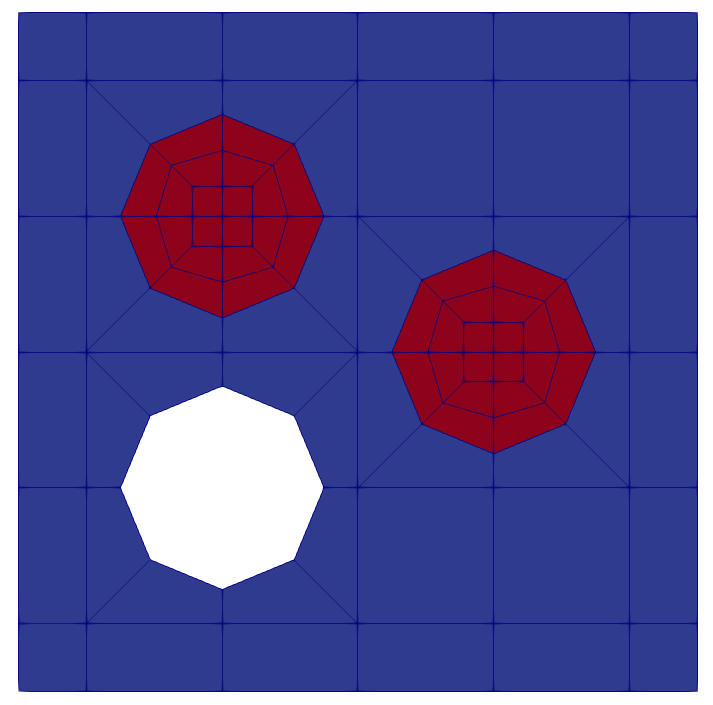
\includegraphics[width=\textwidth]{coarse_mesh.png}
      \caption{2D coarse mesh}
  \end{subfigure}
  \begin{subfigure}[b]{0.45\textwidth}
    \centering
    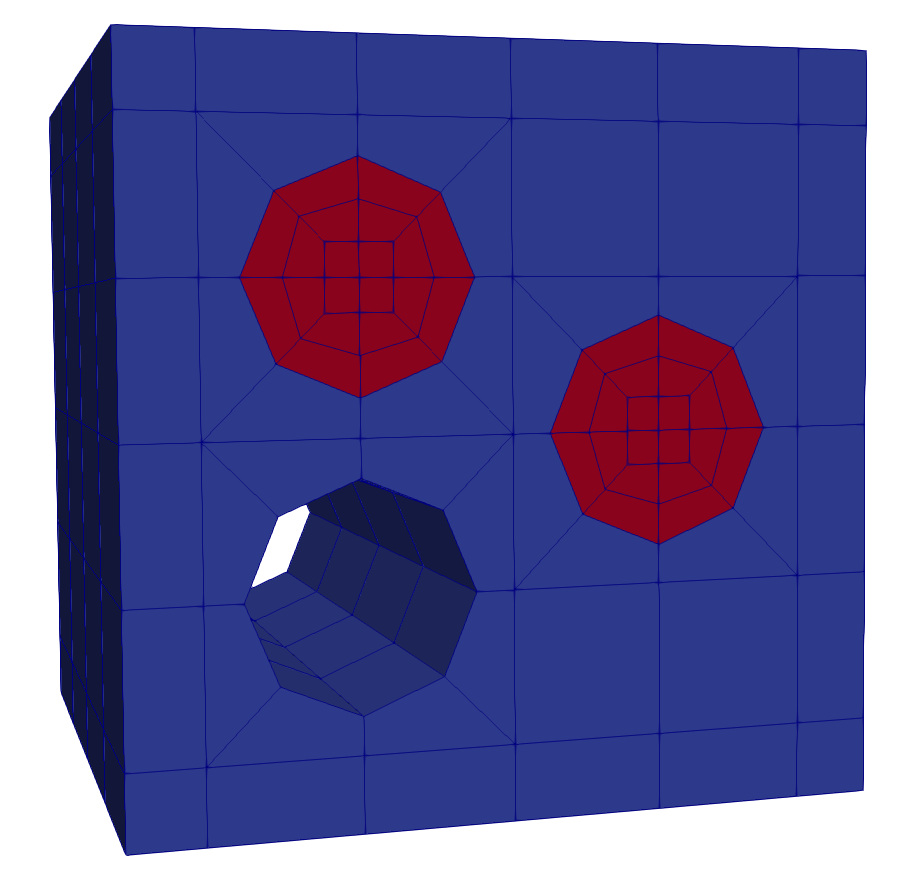
\includegraphics[width=\textwidth]{coarse_mesh_3d.png}
    \caption{3D coarse mesh}
  \end{subfigure}
  \caption{Discretization of the heterogeneous material at the coarsest mesh level.}%
  \label{fig:miehe}
\end{figure}

In this section, we apply the proposed matrix-free operator algorithms for finite-strain hyperelastic material as well as the geometric multigrid preconditioner to a benchmark problem from \cite{Miehe2007}. The coarse mesh for the 2D and 3D problems is illustrated in Figure \ref{fig:miehe}. The 2D material consists of a square (depicted in blue), a hole and two spherical inclusions (depicted in red). The size of the square domain is $10^{-3} \rm{mm}$.
The matrix material is taken to have Poisson's ratio $0.3$ and shear modulus $\mu=0.4225 \times 10^6\, \rm{N/mm^2}$. The inclusion is taken to be $100$ times stiffer.
The 3D material is obtained by extrusion of the 2D geometry into the third dimension.
Note that, although a relatively coarse mesh is used at the coarsest multigrid level, the geometry of the inclusions is captured accurately by manifold descriptions of the boundaries and interfaces.
Both domains are fully fixed along the bottom surface and a distributed load is applied at the top in the $(1,0)$ or $(1,1,0)$ direction for the 2D and the 3D problems, respectively.
The distributed load of $0.5\,\rm{N}$ is applied in 5 steps.
With respect to the nonlinear solver, the displacement tolerance of the $\mathcal{\ell}_2$ norm for the Newton update is taken to be $10^{-5}$ whereas the relative and absolute tolerances for the residual forces is $10^{-8}$. The relative convergence criteria for the linear solver is $10^{-6}$.

\begin{figure}[!ht]
  \centering
  \begin{subfigure}[b]{0.8\textwidth}
    \centering
    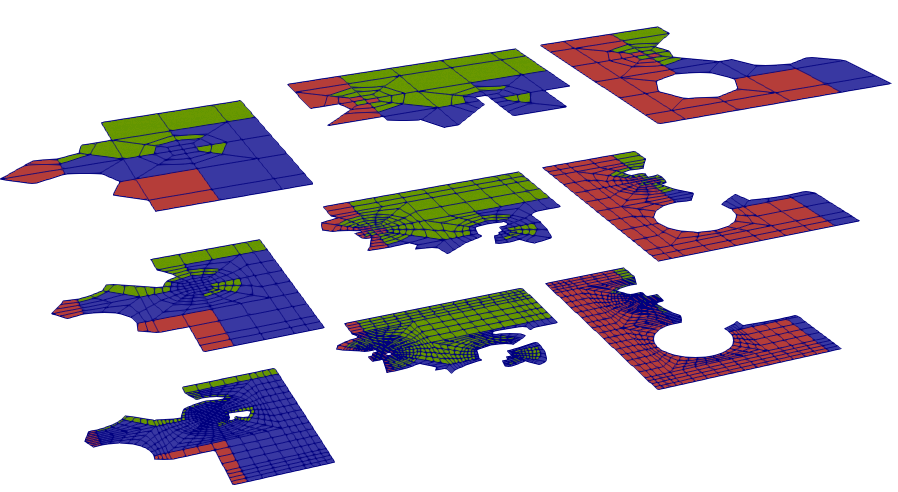
\includegraphics[width=\textwidth]{gmg_2d.png}
    % \caption{2D multigrid mesh with 2 global refinements}
  \end{subfigure}
  \caption{2D multigrid mesh after two global refinements distributed into three MPI processes. Color indicates the process owning the element.}%
  \label{fig:miehe_gmg}
\end{figure}
%
Figure \ref{fig:miehe_gmg} illustrates the hierarchy of multigrid meshes for the 2D problem after two global refinements.

\begin{table}
  \centering
  \begin{tabular}{ccccc}
  \hline
    $p$ & $q$ & $N_{gref}$ & $N_{el}$ & $N_{DoF}$ \\
  \hline
    1 & 2 & 7 & 1441792 & 2887680 \\
    2 & 3 & 6 & 360448 & 2887680 \\
    3 & 4 & 5 & 90112 & 1625088 \\
    4 & 5 & 5 & 90112 & 2887680 \\
    5 & 6 & 5 & 90112 & 4510720 \\
    6 & 7 & 4 & 22528 & 1625088 \\
    7 & 8 & 4 & 22528 & 2211328 \\
    8 & 9 & 4 & 22528 & 2887680 \\
  \hline
  \end{tabular}
  \caption{Parameters for the 2D benchmark: $p$ is the polynomial degree,
  $q$ is the quadrature order, $N_{gref}$ is the number of global mesh refinements, $N_{el}$ is the number of elements and $N_{DoF}$ is the number of DoFs.
  }
  \label{tab:input_parameters_2d}
\end{table}

\begin{table}
  \centering
  \begin{tabular}{ccccc}
  \hline
    $p$ & $q$ & $N_{gref}$ & $N_{el}$ & $N_{DoF}$ \\
  \hline
    1 & 2 & 4 & 1441792 & 4442880 \\
    2 & 3 & 3 & 180224 & 4442880 \\
    3 & 4 & 2 & 22528 & 1891008 \\
    4 & 5 & 2 & 22528 & 4442880 \\
  \hline
  \end{tabular}
  \caption{Parameters for the 3D benchmark: $p$ is the polynomial degree,
  $q$ is the quadrature order, $N_{gref}$ is the number of global mesh refinements, $N_{el}$ is the number of elements and $N_{DoF}$ is the number of DoFs.
  }
  \label{tab:input_parameters_3d}
\end{table}

The benchmark calculations are performed for 2D and 3D problems with various combination of polynomial degrees and number of global refinements, as is stated in Tables \ref{tab:input_parameters_2d} and \ref{tab:input_parameters_3d}.
Shared memory parallelization using Intel Threading Building Blocks was disabled for this study.
%

We are interested in the following metrics:
\begin{itemize}
\item the wall-clock time and memory requirement per DoF for matrix-vector multiplication;
\item the average number of CG iterations throughout the entire simulation (i.e. each Newton-Raphson iteration and each loading step);
\item the wall-clock time per DoF for the CG solver;
\end{itemize}
%
The results of the matrix-free approach with a geometric-multigrid preconditioner are compared to the matrix-based approach in conjunction with the algebraic multigrid (AMG) preconditioner using the package ML of the Trilinos \cite{Heroux2005} library, version 12.12.1.
The aggregation threshold for the AMG preconditioner is taken as $10^{-4}$.
Computations are done on a single node of two clusters:
A node on the ``Emmy'' cluster at RRZE, FAU has two Xeon 2660v2 ``Ivy Bridge'' chips (10 cores per chip + SMT) running at 2.2 GHz with 25 MB shared cache per chip and 64 GB of RAM. Intel's compiler version 18.03 with flags ``-O3 -march=native'' and Intel MPI version 18.03 are used.
The ``IWR'' results were obtained on a single machine with eight Xeon E7-8870 ``Sandy Bridge'' chips (10 cores per chip  + SMT) running at 2.4 GHz with 30 MB shared cache per chip. For the simulation, GCC version 8.1.0 with flags ``-O3 -march=native'' and OpenMPI version 3.0.0 were used.

\subsection{Matrix-vector multiplication}

\begin{figure}[!ht]
  \centering
  \begin{subfigure}[b]{0.49\textwidth}
      \centering
      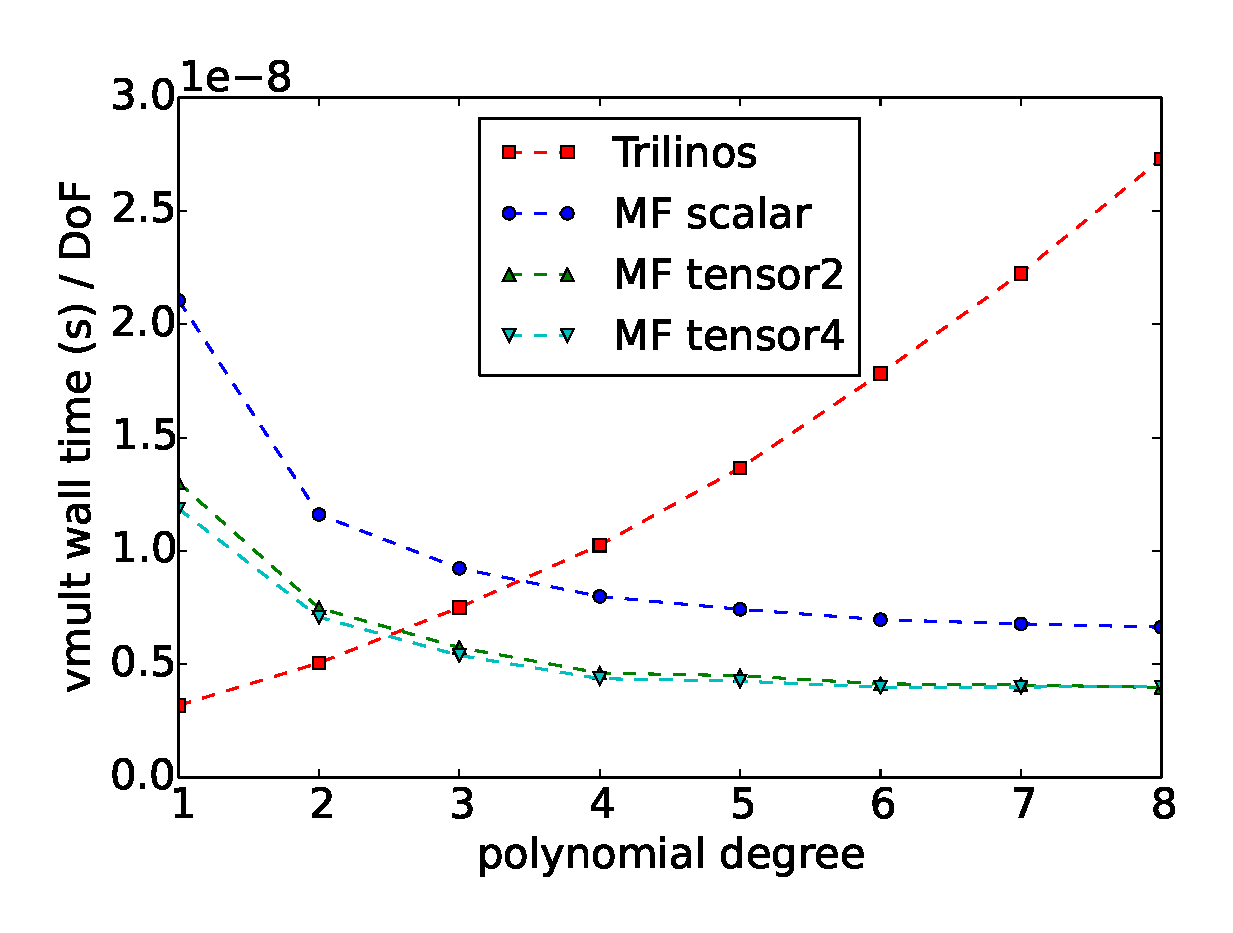
\includegraphics[width=\textwidth]{Emmy_RRZE_timing2d.eps}
      \caption{matrix-vector product (2D)}
      \label{fig:benchmark_miehe_Emmy_vmult2}
  \end{subfigure}
  \begin{subfigure}[b]{0.49\textwidth}
    \centering
    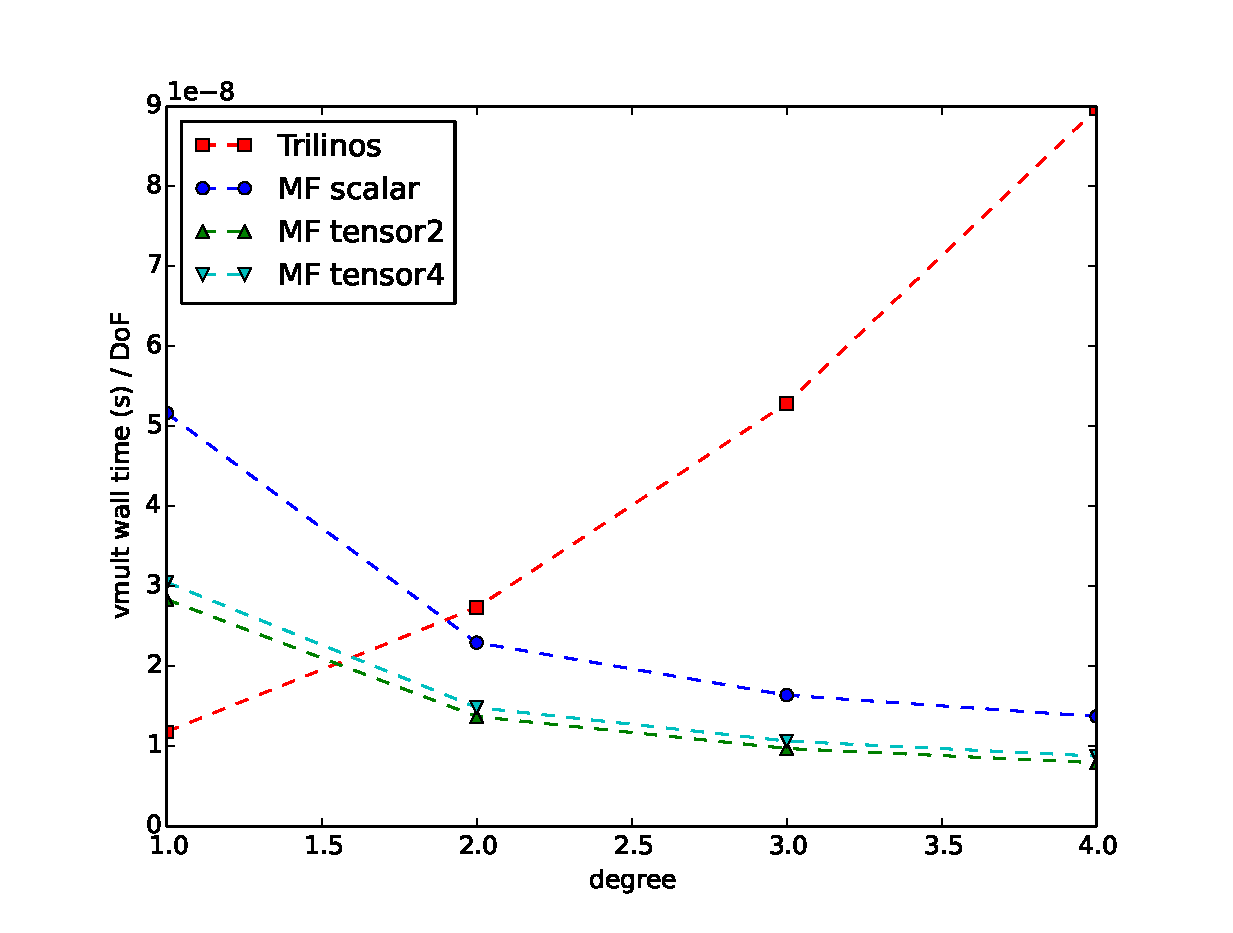
\includegraphics[width=\textwidth]{Emmy_RRZE_timing3d.eps}
    \caption{matrix-vector product (3D)}
    \label{fig:benchmark_miehe_Emmy_vmult3}
  \end{subfigure}
  ~
  \begin{subfigure}[b]{0.49\textwidth}
      \centering
      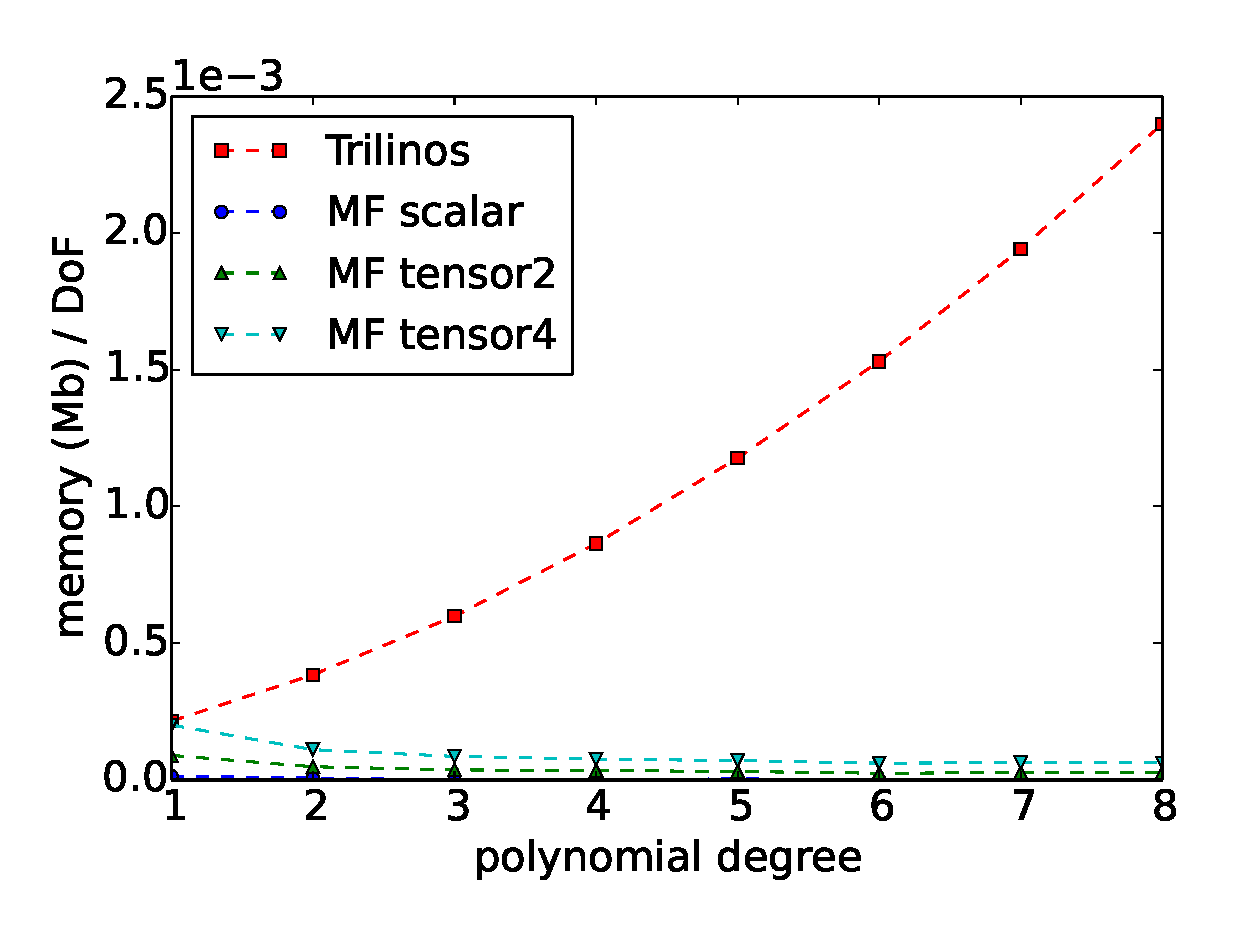
\includegraphics[width=\textwidth]{Emmy_RRZE_memory2d.eps}
      \caption{memory consumption (2D)}
      \label{fig:benchmark_miehe_Emmy_memory2}
  \end{subfigure}
  \begin{subfigure}[b]{0.49\textwidth}
    \centering
    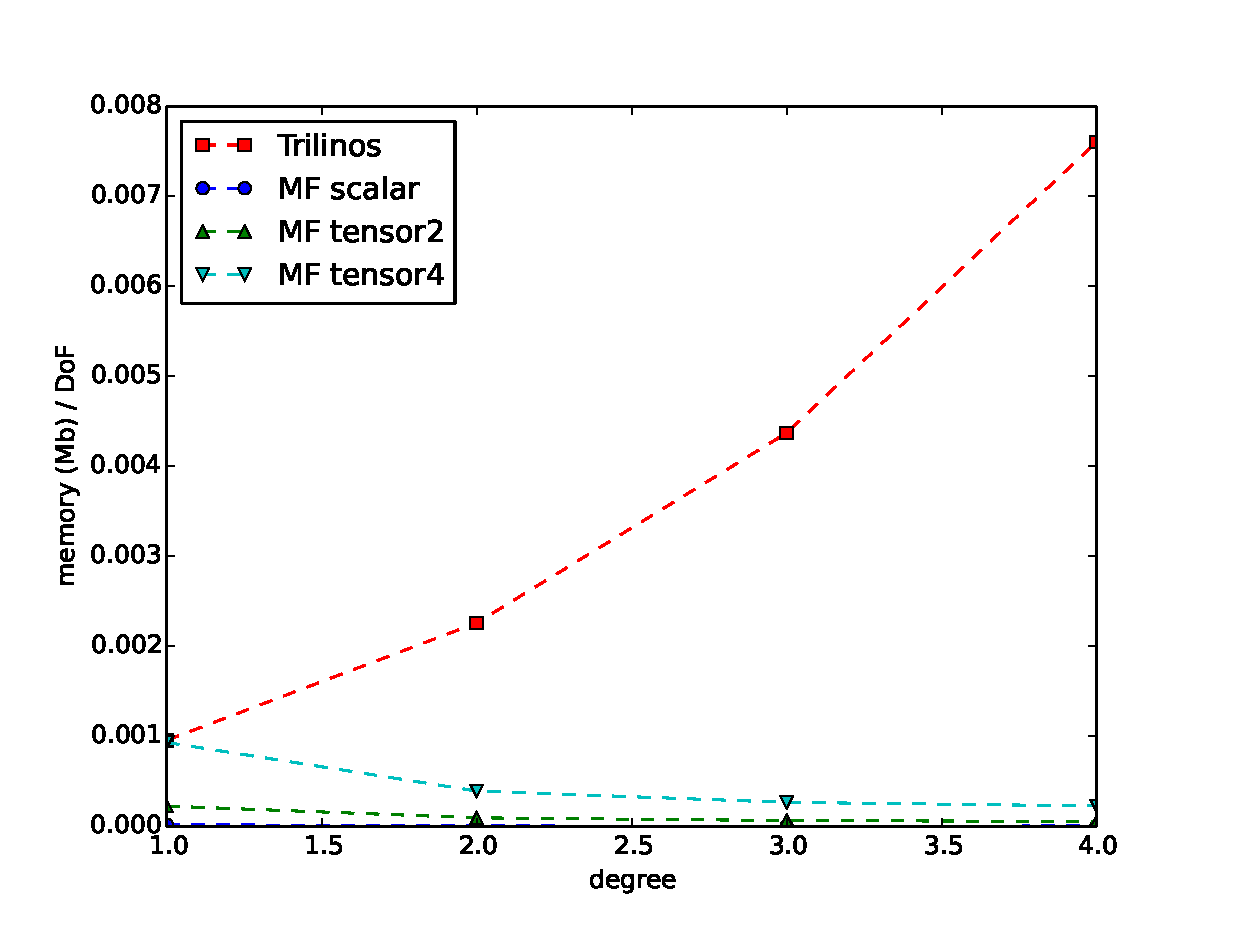
\includegraphics[width=\textwidth]{Emmy_RRZE_memory3d.eps}
    \caption{memory consumption (3D)}
    \label{fig:benchmark_miehe_Emmy_memory3}
  \end{subfigure}
  \caption{Emmy cluster, RRZE, matrix-vector multiplication.}%
  \label{fig:benchmark_miehe_Emmy}
\end{figure}

\begin{figure}[!ht]
  \centering
  \begin{subfigure}[b]{0.49\textwidth}
      \centering
      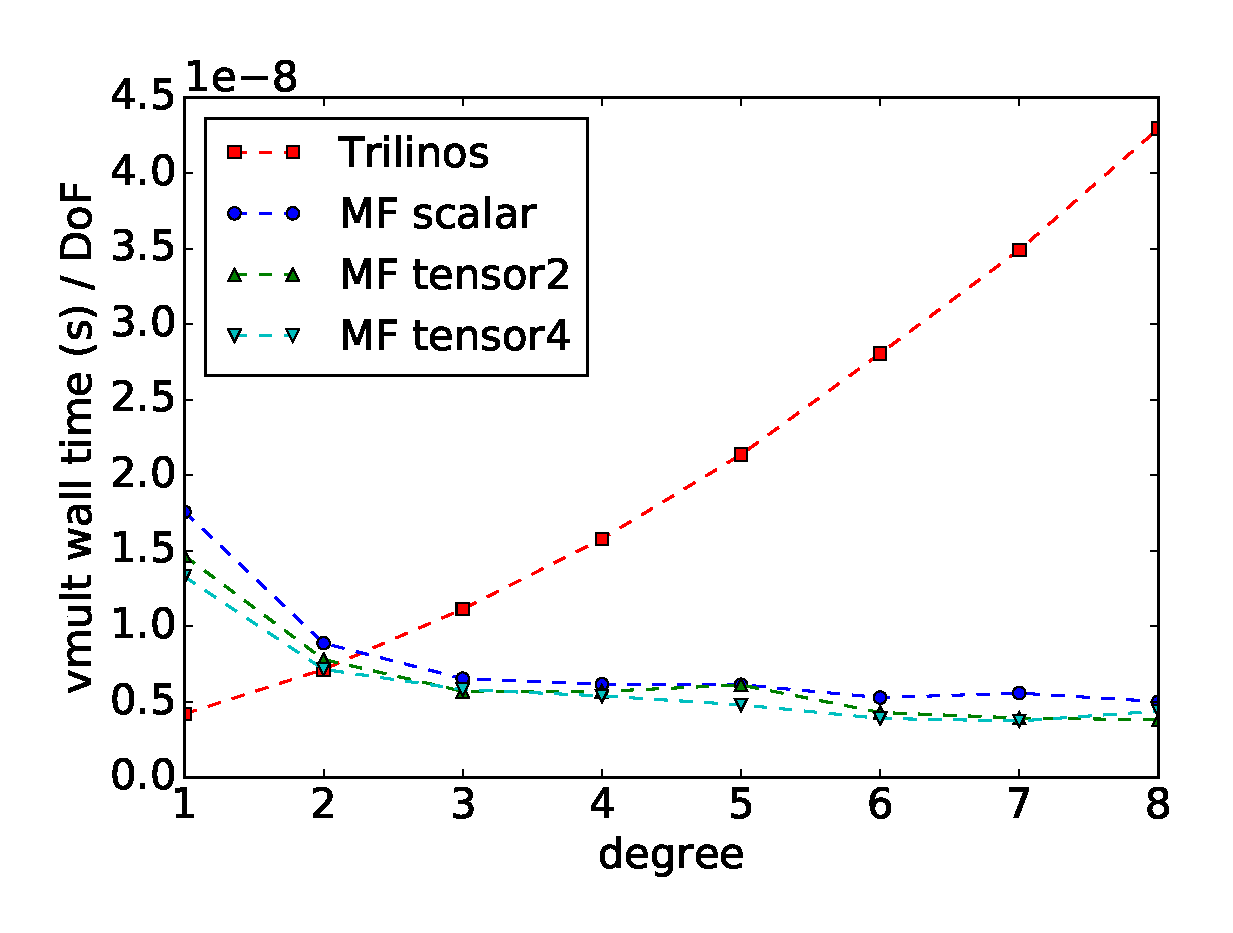
\includegraphics[width=\textwidth]{IWR_timing2d.eps}
      \caption{matrix-vector product (2D)}
      \label{fig:benchmark_miehe_IWR_vmult2}
  \end{subfigure}
  \begin{subfigure}[b]{0.49\textwidth}
    \centering
    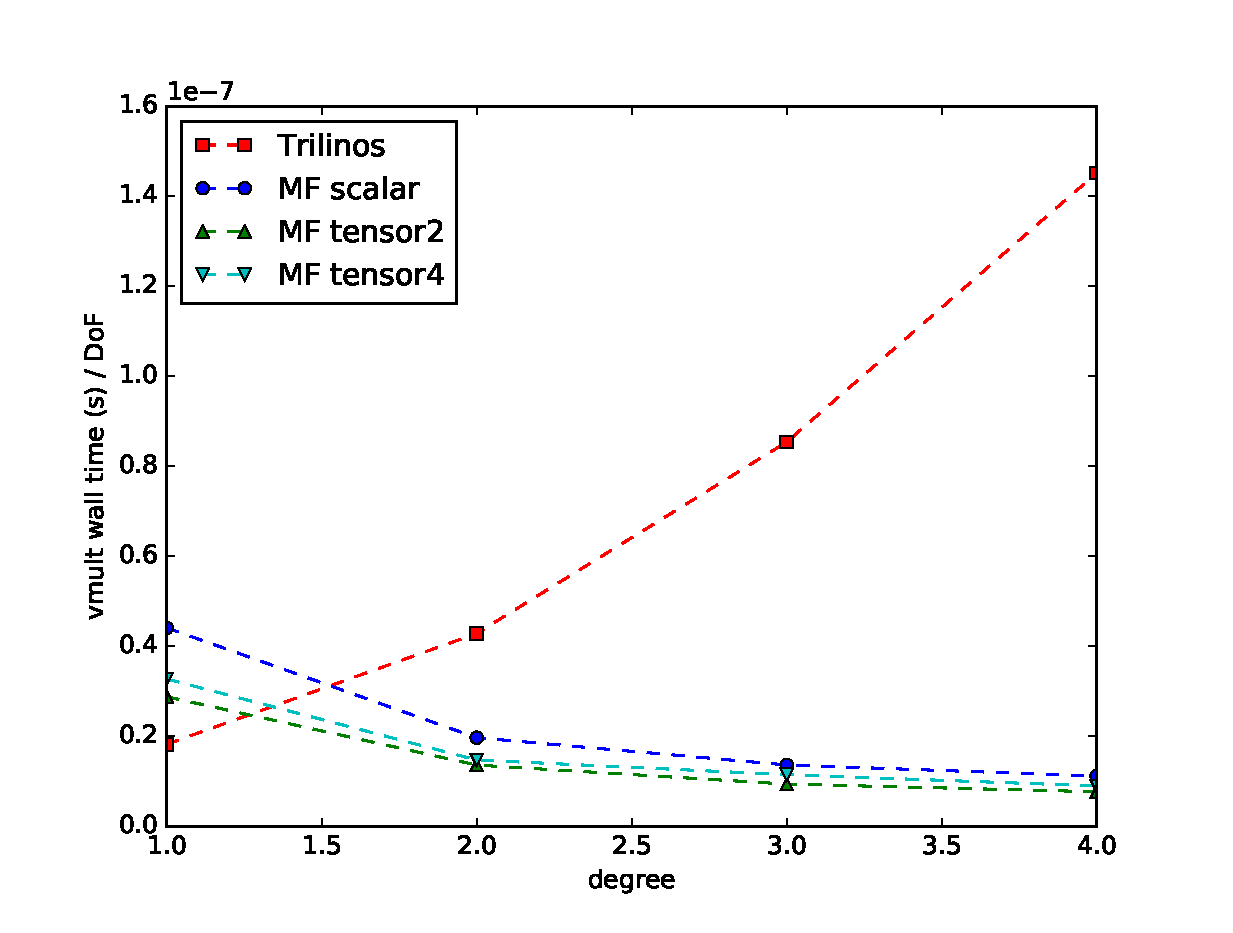
\includegraphics[width=\textwidth]{IWR_timing3d.eps}
    \caption{matrix-vector product (3D)}
    \label{fig:benchmark_miehe_IWR_vmult3}
  \end{subfigure}
  ~
  \begin{subfigure}[b]{0.49\textwidth}
      \centering
      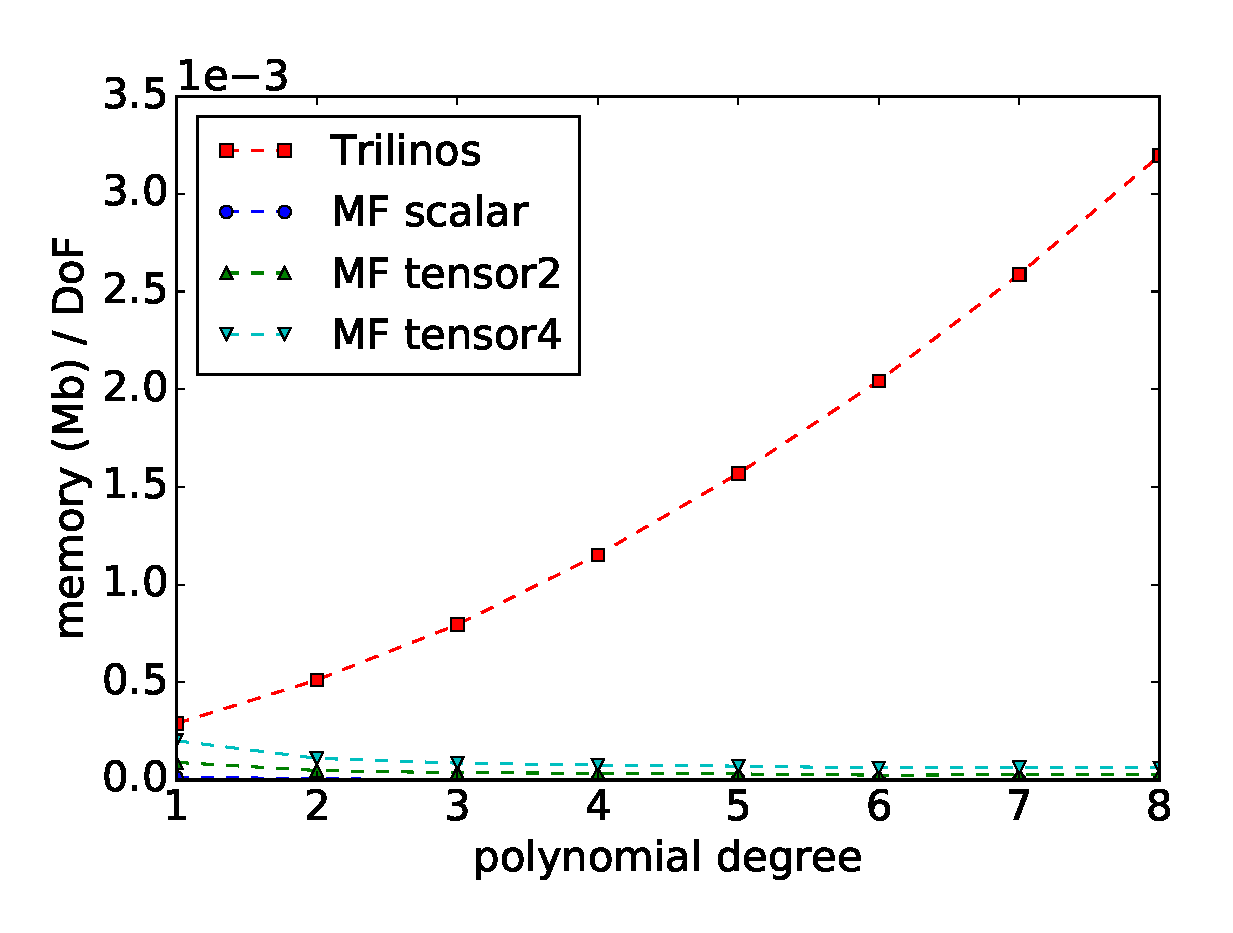
\includegraphics[width=\textwidth]{IWR_memory2d.eps}
      \caption{memory consumption (2D)}
      \label{fig:benchmark_miehe_IWR_memory2}
  \end{subfigure}
  \begin{subfigure}[b]{0.49\textwidth}
    \centering
    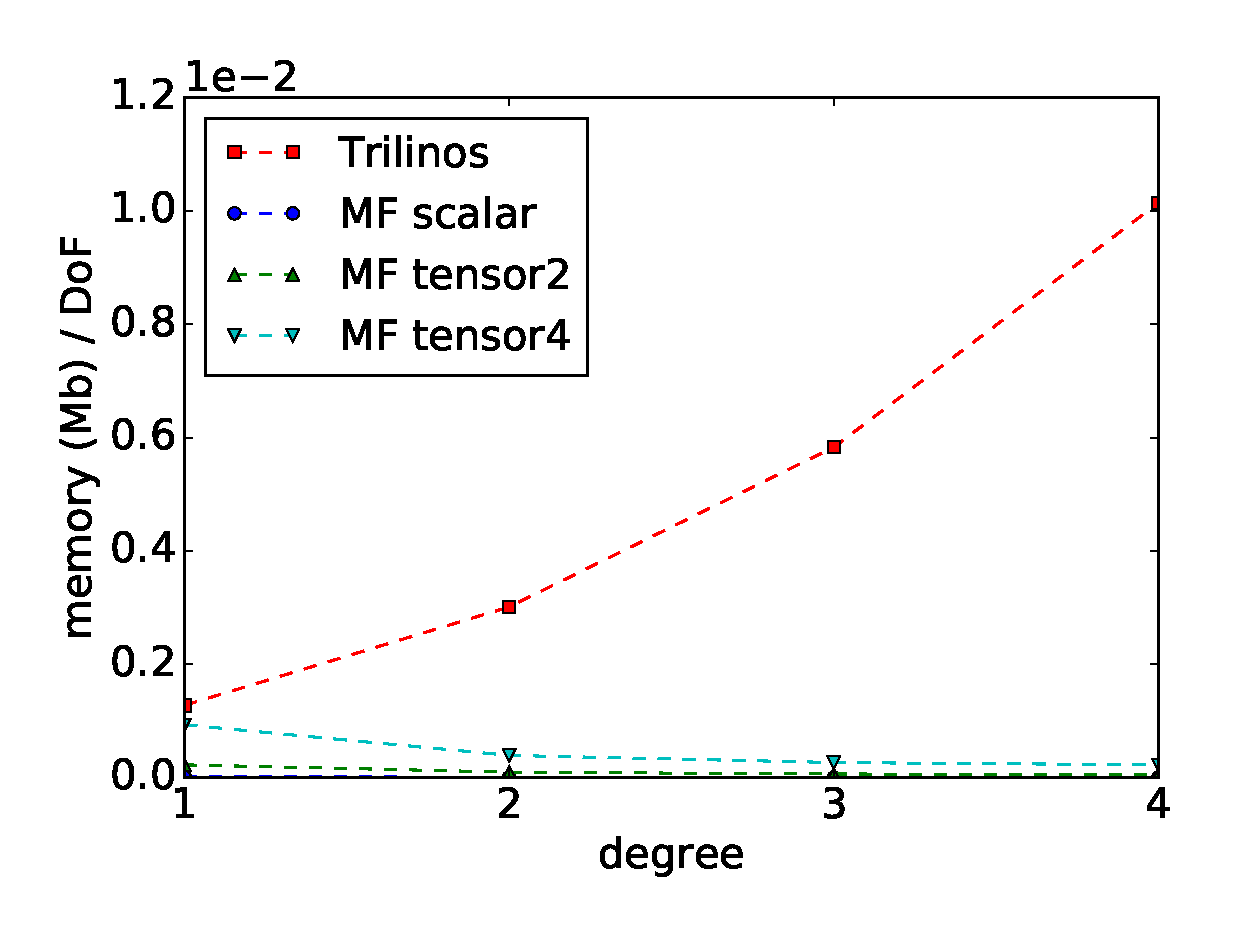
\includegraphics[width=\textwidth]{IWR_memory3d.eps}
    \caption{memory consumption (3D)}
    \label{fig:benchmark_miehe_IWR_memory3}
  \end{subfigure}
  \caption{IWR cluster, matrix-vector multiplication}%
  \label{fig:benchmark_miehe_IWR}
\end{figure}

Figures \ref{fig:benchmark_miehe_Emmy} and \ref{fig:benchmark_miehe_IWR} show the results of the matrix-vector multiplication benchmarks as performed on the two clusters.
As expected, the matrix-vector multiplication becomes very expensive for higher order discretization for sparse matrix-based approaches.
The matrix-free implementation is faster than the matrix-based counterpart already for cubic Lagrangian basis in 2D and quadratic in 3D.
Figures \ref{fig:benchmark_miehe_Emmy_vmult2}, \ref{fig:benchmark_miehe_Emmy_vmult3}, \ref{fig:benchmark_miehe_IWR_vmult2} and \ref{fig:benchmark_miehe_IWR_vmult3} clearly show the influence of the different caching strategies.
Two conclusions can be drawn from these results:
The scalar caching implementation is the most time consuming of the three, as at each step we additionally evaluate the gradient of the displacement field in the reference configuration that is required to evaluate the Kirchhoff stress $\gz \tau$.
There is little difference between the approach where the fourth-order material tangent tensor is cached (``tensor4'') and the one where we only cache the second-order Kirchhoff tensor and utilize the chosen hyperelastic constitutive equation to efficiently implement the action of the material tangent on the second-order symmetric tensor.
This indicates that the time savings we get from the latter approach are insignificant within the complete matrix-free operator implementation.
Consequently, we can apply the matrix-free approach to any finite-strain material model by caching the fourth-order material tangent in addition to the Kirchhoff stress and expect this to be faster than the matrix-based implementation.
It is therefore feasible to define highly performant generic operators that are independent of any applied constitutive laws.

As outlined in the introduction, it is not only the performance of the matrix-free vector multiplication, but also the memory requirement to store a sparse matrix which is the driving force behind matrix-free methods.
Figures \ref{fig:benchmark_miehe_Emmy_memory2}, \ref{fig:benchmark_miehe_Emmy_memory3}, \ref{fig:benchmark_miehe_IWR_memory2} and \ref{fig:benchmark_miehe_IWR_memory3} demonstrate that even with caching one fourth-order symmetric tensor and one second-order tensor at each quadrature point, the matrix-free approach takes much less memory than its matrix-based counterpart.

\subsection{Preconditioned iterative solver}

\begin{figure}[!ht]
  \begin{subfigure}[b]{0.49\textwidth}
    \centering
    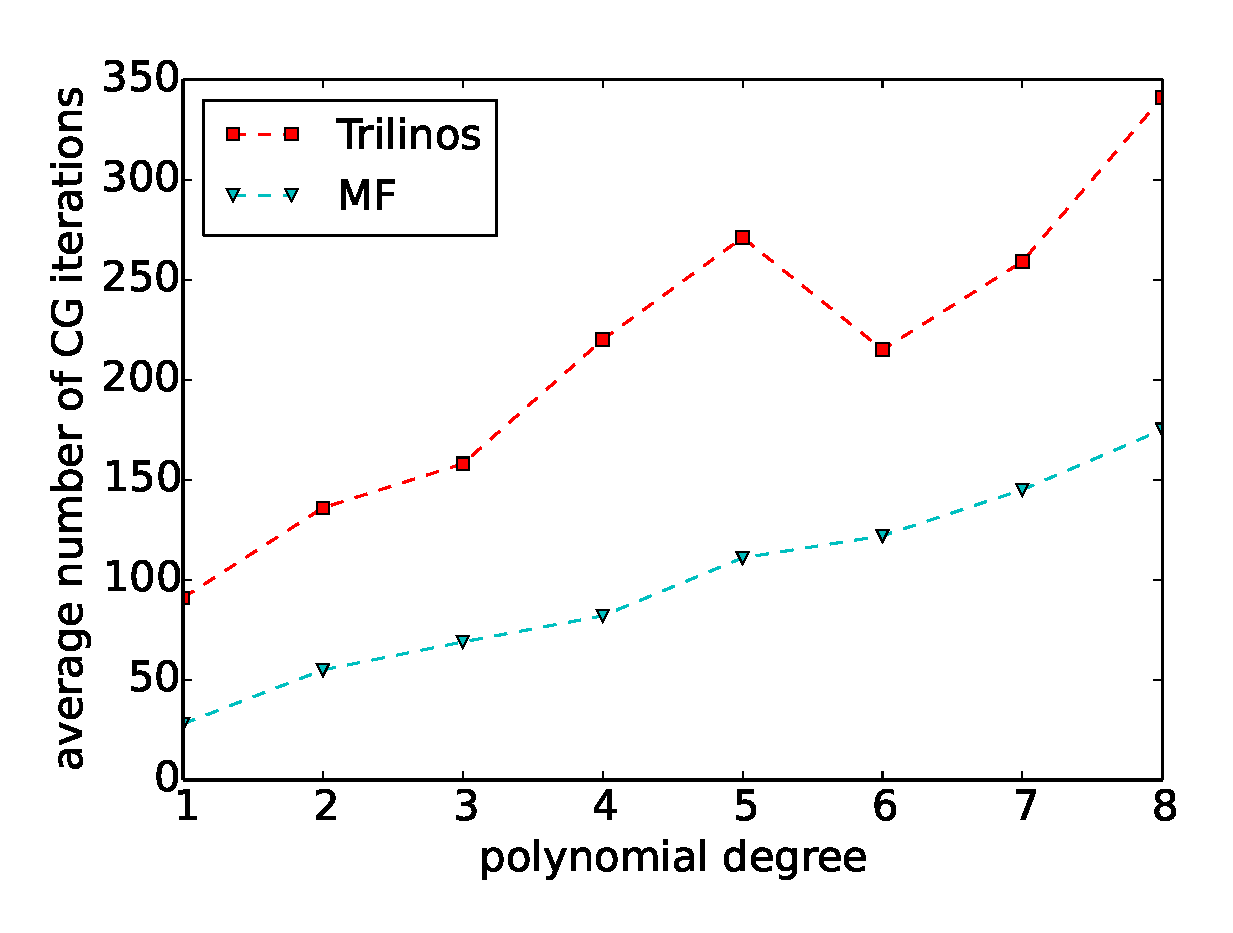
\includegraphics[width=\textwidth]{Emmy_RRZE_cg2d.eps}
    \caption{CG iterations (2D)}
    \label{fig:benchmark_miehe_Emmy_cg2}
  \end{subfigure}
  \begin{subfigure}[b]{0.49\textwidth}
    \centering
    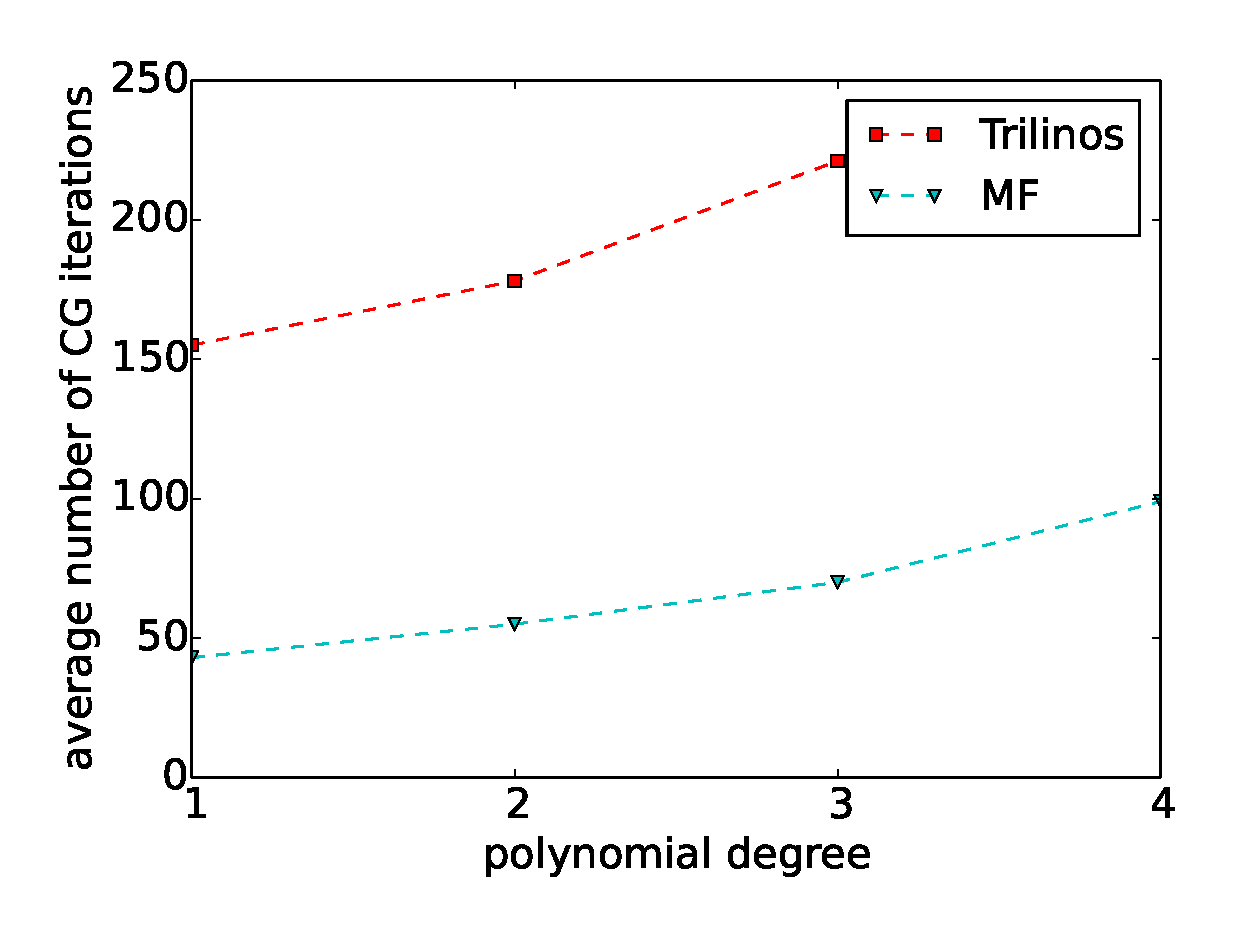
\includegraphics[width=\textwidth]{Emmy_RRZE_cg3d.eps}
    \caption{CG iterations (3D)}
    \label{fig:benchmark_miehe_Emmy_cg3}
  \end{subfigure}
  ~
  \begin{subfigure}[b]{0.49\textwidth}
    \centering
    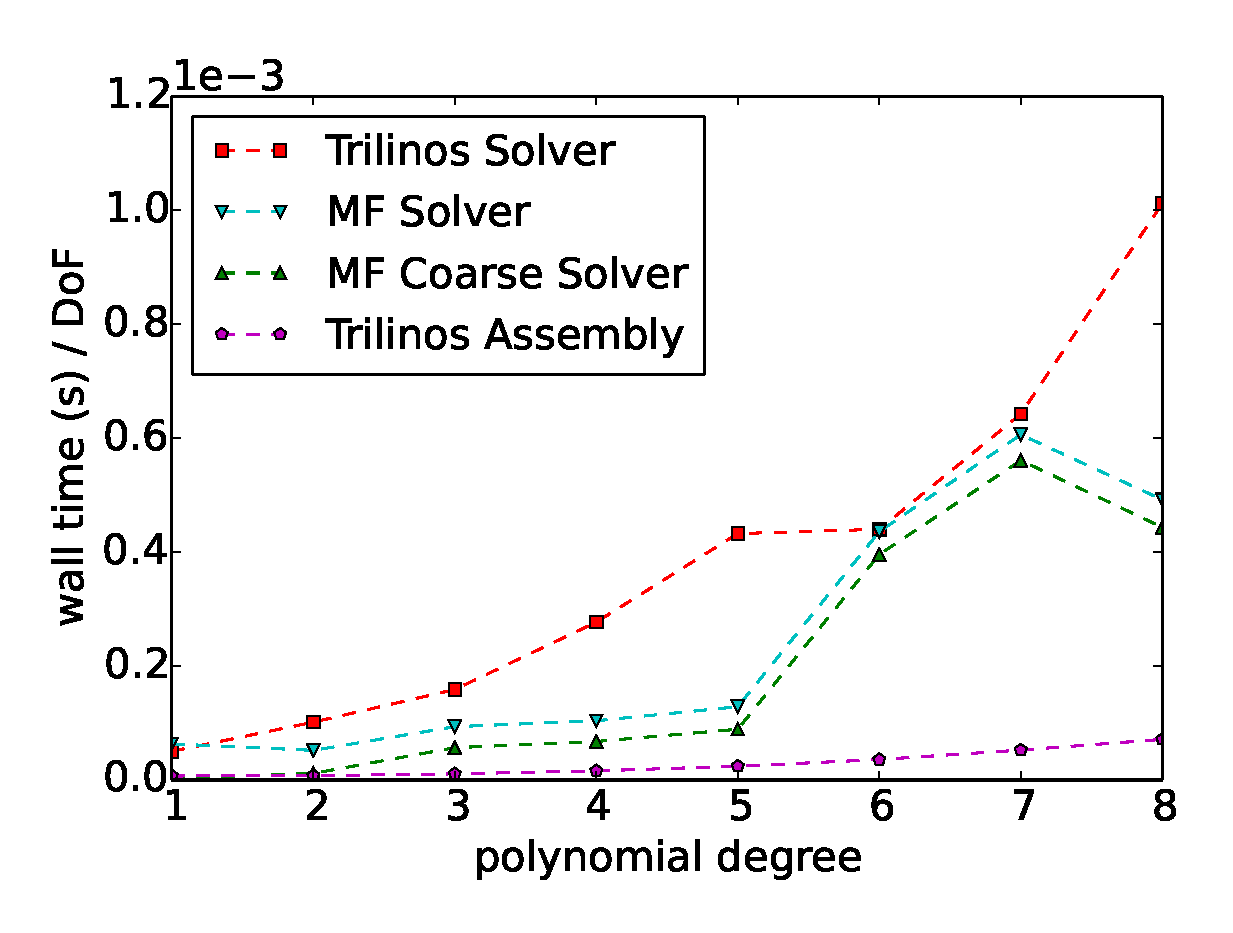
\includegraphics[width=\textwidth]{Emmy_RRZE_solver2d.eps}
    \caption{CG solution time (2D)}
    \label{fig:benchmark_miehe_Emmy_sol2}
  \end{subfigure}
  \begin{subfigure}[b]{0.49\textwidth}
    \centering
    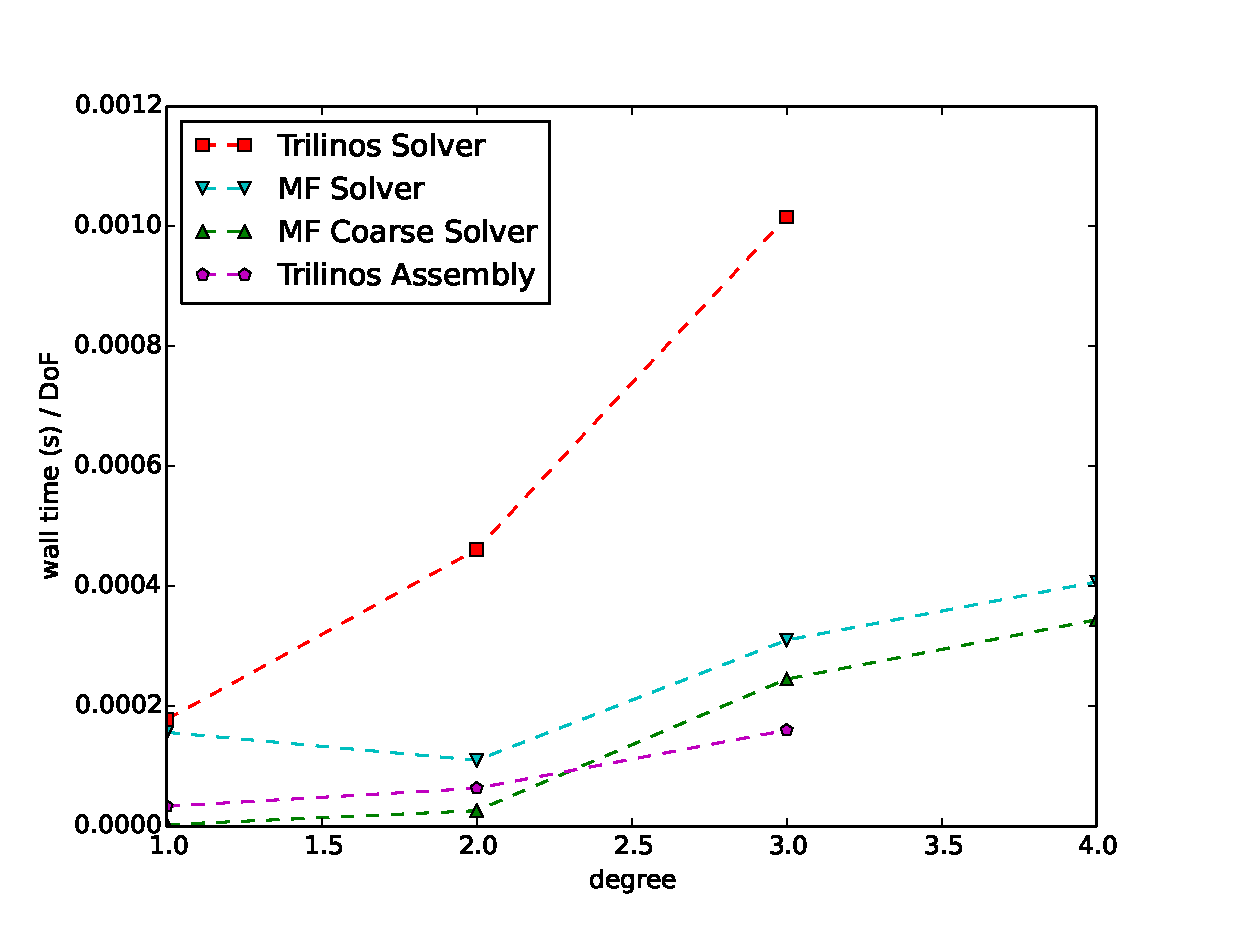
\includegraphics[width=\textwidth]{Emmy_RRZE_solver3d.eps}
    \caption{CG solution time (3D)}
    \label{fig:benchmark_miehe_Emmy_sol3}
  \end{subfigure}
  \caption{Emmy cluster, RRZE, iterative solver.}%
  \label{fig:benchmark_miehe_Emmy_cg}
\end{figure}

\begin{figure}[!ht]
  \begin{subfigure}[b]{0.49\textwidth}
    \centering
    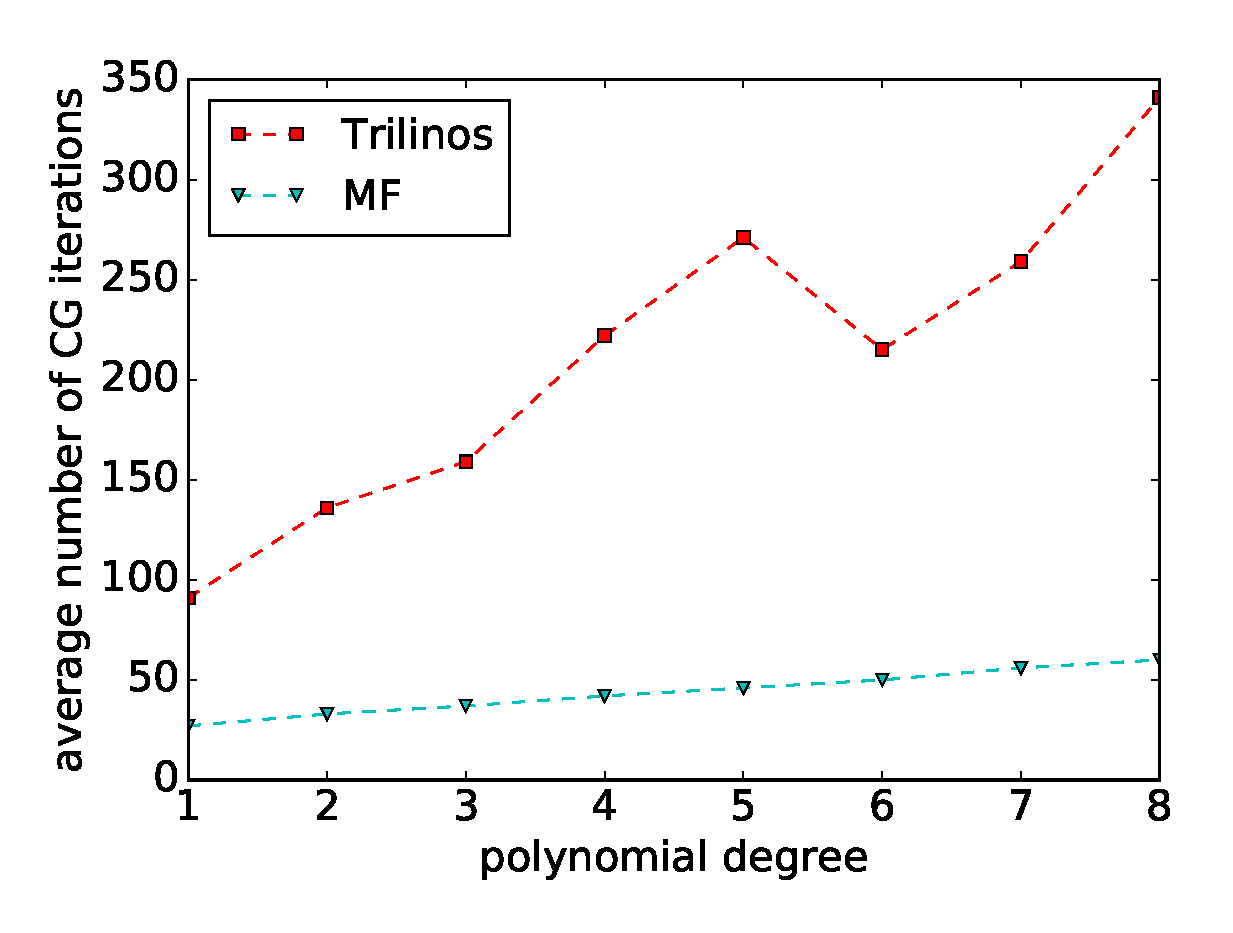
\includegraphics[width=\textwidth]{IWR_cg2d.eps}
    \caption{CG iterations (2D)}
    \label{fig:benchmark_miehe_IWR_cg2}
  \end{subfigure}
  \begin{subfigure}[b]{0.49\textwidth}
    \centering
    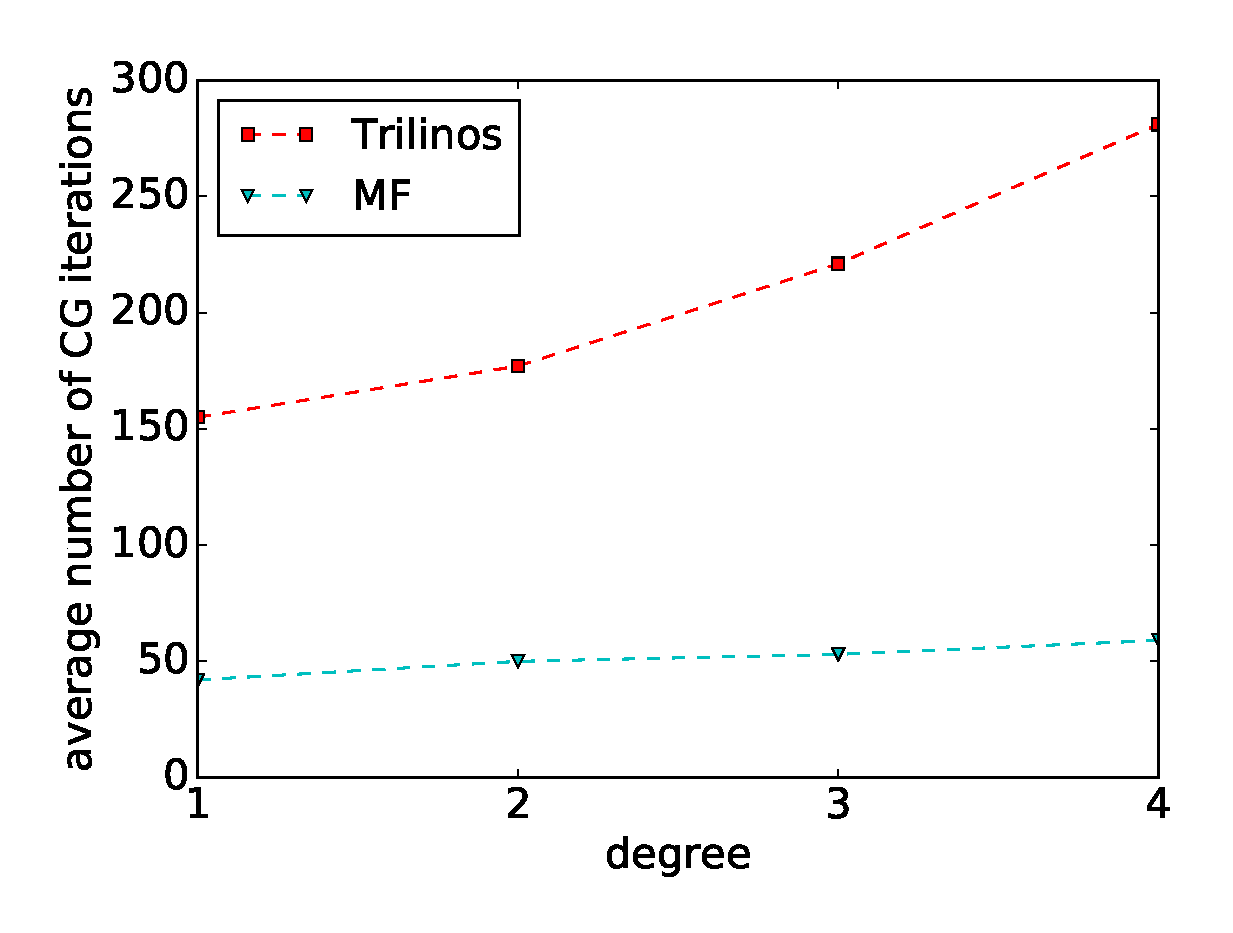
\includegraphics[width=\textwidth]{IWR_cg3d.eps}
    \caption{CG iterations (3D)}
    \label{fig:benchmark_miehe_IWR_cg3}
  \end{subfigure}
  ~
  \begin{subfigure}[b]{0.49\textwidth}
    \centering
    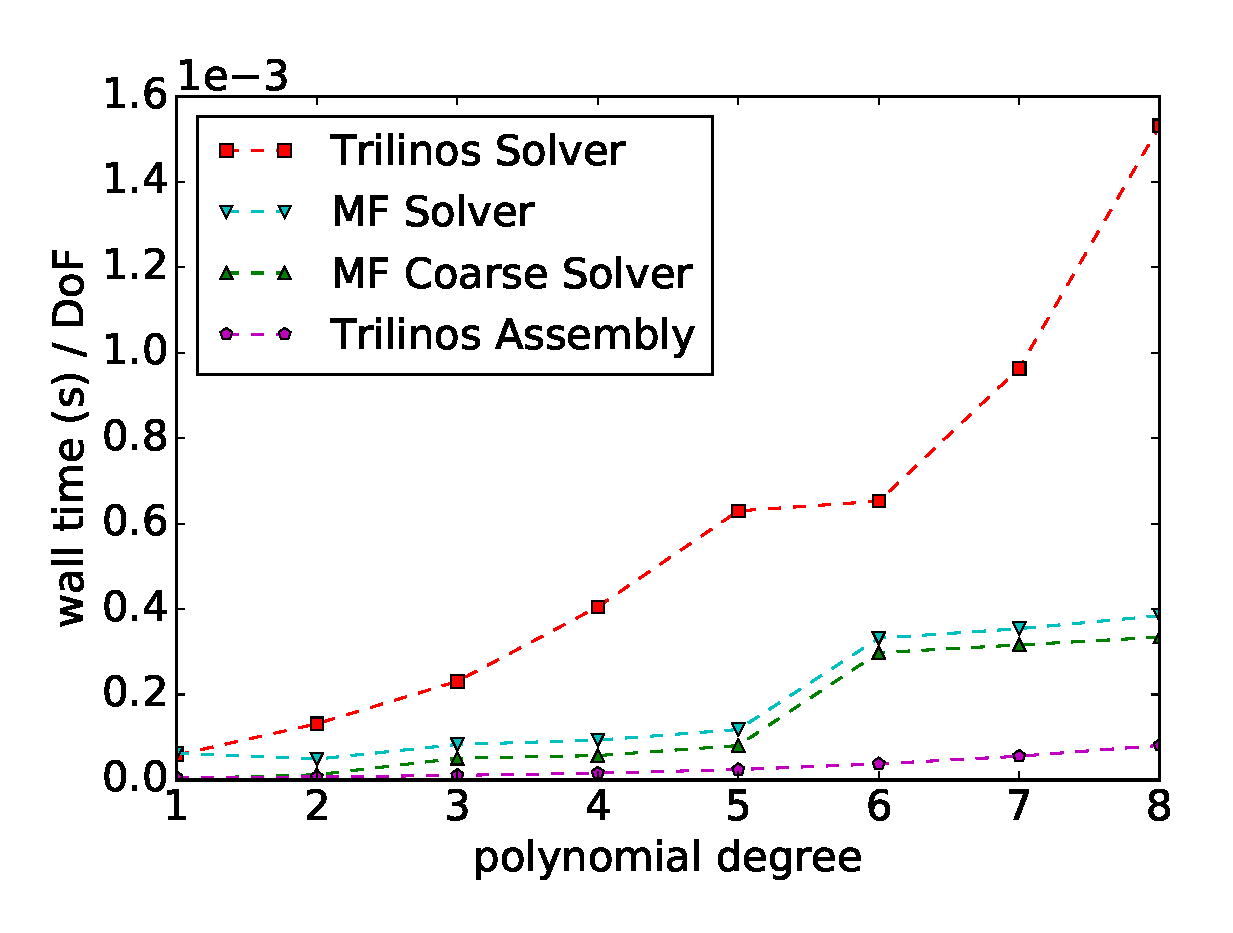
\includegraphics[width=\textwidth]{IWR_solver2d.eps}
    \caption{CG solution time (2D)}
    \label{fig:benchmark_miehe_IWR_sol2}
  \end{subfigure}
  \begin{subfigure}[b]{0.49\textwidth}
    \centering
    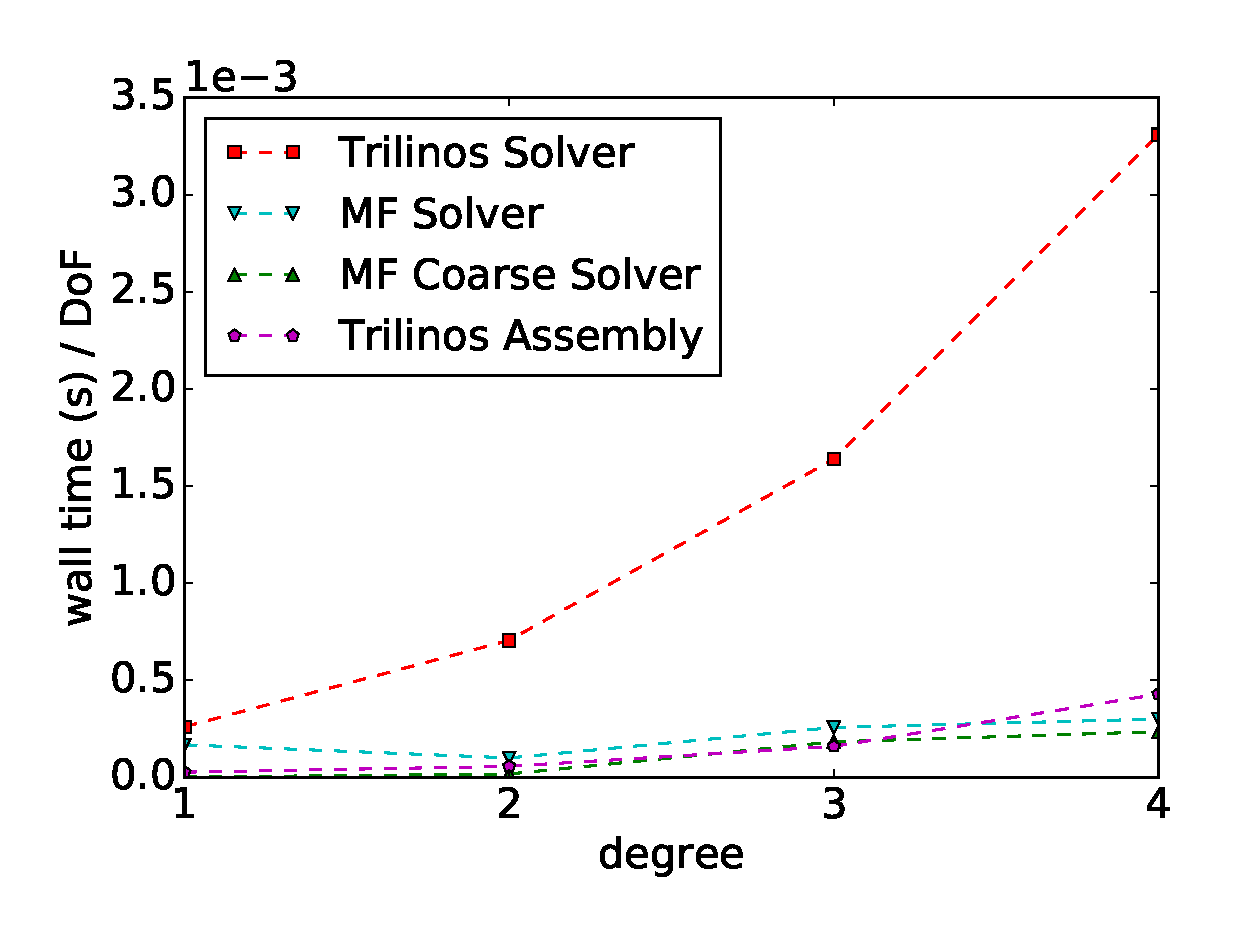
\includegraphics[width=\textwidth]{IWR_solver3d.eps}
    \caption{CG solution time (3D)}
    \label{fig:benchmark_miehe_IWR_sol3}
  \end{subfigure}
  \caption{IWR cluster.}%
  \label{fig:benchmark_miehe_IWR_cg}
\end{figure}

Next we evaluate the performance of the proposed geometric multigrid preconditioner.
First we consider the number of iterations in the conjugate gradient (CG) solver.
Figures \ref{fig:benchmark_miehe_Emmy_cg2}, \ref{fig:benchmark_miehe_Emmy_cg3}, \ref{fig:benchmark_miehe_IWR_cg2} and \ref{fig:benchmark_miehe_Emmy_cg3} show a very mild increase in the average number of CG iterations for different polynomial degrees.
On the other hand, the black-box AMG preconditioner requires many more iterations for convergence.
Figures \ref{fig:benchmark_miehe_Emmy_sol2}, \ref{fig:benchmark_miehe_Emmy_sol3}, \ref{fig:benchmark_miehe_IWR_sol2} and \ref{fig:benchmark_miehe_IWR_sol3} confirm that the efficiency of the proposed GMG preconditioner translates into faster solution times for polynomial degrees up to $p=5$.
For higher orders in 2D the wall-clock time is comparable to the AMG preconditioner, see Figure \ref{fig:benchmark_miehe_Emmy_sol2}.
The reason for this is the suboptimal coarse level solver within the GMG preconditioner.
Evidently, the combination of the Chebyshev smoother with the CG solver at the coarsest mesh level has unsatisfactory performance for higher polynomial degrees.
One possible solution to this issues would be to perform further coarsening combined with the homogenization-based transfer operators \cite{Miehe2007}.
Although untested in this work, we hypothesize that this should also improve the performance of the preconditioner for lower degrees.
A valid alternative would be to use matrix-based AMG at the coarsest level.

\section{Summary and Conclusions}
\label{sec:summary}

In this contribution, we proposed and numerically investigated several matrix-free implementations of tangent operators for finite-strain elasticity with heterogeneous materials.
The implementation that caches the fourth-order material tangent together with the second-order Kirchhoff stress was shown to be faster than the matrix-based approach for quadratic elements in 3D and cubic in 3D.
This gives hope that the matrix-free implementation of the tangent operator can be applied to any constitutive model which operates with the material tangent on the quadrature point level.

We also studied the performance of the GMG preconditioner with standard geometric transfer operations between each level.
The GMG was applied to heterogeneous material assuming that the coarsest level can provide an adequate discretization of the heterogeneity.
The numerical studies indicate that the proposed preconditioner leads to a solution approach that is faster than the matrix-based AMG for moderately high polynomial degrees (approximately up to order five).
However, a considerable amount of time of GMG preconditioner is spent in the coarse level solver.
Our future work will, therefore, be focused on extending the proposed matrix-free multigrid solution approach to homogenization based transfer operators \cite{Miehe2007}.
We are also interested in extending these methods to near incompressible three-field formulations.

\section*{Acknowledgements}

D.~Davydov acknowledge the financial support of the German Research Foundation (DFG), grant DA 1664/2-1.

D.~Davydov, D.~Arndt and J-P.~Pelteret are grateful to Jed Brown (CU Boulder) and Veselin Dobrev (Lawrence Livermore National Laboratory) for a fruitful discussion on matrix-free operator evaluation approaches.

D.~Arndt was supported by the German Research Foundation (DFG) under the project ``High-order discontinuous
Galerkin for the exa-scale'' (\mbox{ExaDG}) within the priority program ``Software
for Exascale Computing'' (SPPEXA).

% J-P.~Pelteret was supported by the European Research Council (ERC) through
% the Advanced Grant 289049 MOCOPOLY

P.~Steinmann acknowledges the support of the Cluster of Excellence Engineering of Advanced Materials (EAM) which made this collaboration possible.

\section*{Bibliography}

\bibliographystyle{elsarticle-num}
\bibliography{bibliography}

\end{document}
